\documentclass[aspectratio=169]{beamer}

\usepackage{lmodern}
\usepackage{hyperref}
\usepackage{graphicx}
\usepackage{tikz}
\usepackage{amsmath}
\usepackage{booktabs}
\usepackage{array}
\usepackage{tabularx}
\usetikzlibrary{positioning}

\graphicspath{{../results/}{../specification/}}

% ----- Theme -----
\definecolor{MainPink}{HTML}{C2185B}
\definecolor{DarkPink}{HTML}{880E4F}
\definecolor{SoftPink}{HTML}{F8BBD0}
\definecolor{DarkGray}{HTML}{2E2E2E}
\definecolor{NavyBlue}{HTML}{1A237E}

\setbeamercolor{structure}{fg=MainPink}
\setbeamercolor{frametitle}{fg=white,bg=MainPink}
\setbeamercolor{title}{fg=white,bg=MainPink}
\setbeamercolor{block title}{fg=white,bg=DarkPink}
\setbeamercolor{block body}{bg=SoftPink,fg=DarkGray}

\setbeamertemplate{navigation symbols}{}

% ---------- Section divider helper ----------
\newcommand{\sectiondivider}[4]{%
  % #1 part number  #2 part title  #3 presenter name  #4 slides covered
  \begin{frame}[plain]
  \begin{tikzpicture}[remember picture, overlay]
    \fill[DarkPink] (current page.south west) rectangle (current page.north east);
    \node[anchor=north west, font=\Large\bfseries\color{SoftPink}]
      at ([xshift=1.2cm, yshift=-1.0cm] current page.north west) {#1};
    \node[anchor=center, font=\LARGE\bfseries\color{white}, text width=0.75\paperwidth, align=center]
      at (current page.center) {#2};
    \node[anchor=south, font=\small\color{white!70!DarkPink}]
      at ([yshift=1.0cm] current page.south) {#4};
  \end{tikzpicture}
  \end{frame}
}

\title{Wind-Assisted Propulsion on North Sea Routes\\
\normalsize Maritime Performance Analytics for Flettner Rotors}
\author{Aleksandra K\l{}os \quad Olga Grigorieva \quad Elen Mouradian \quad Bartosz Maj \quad Hubert Jaczy\'nski}
\institute{DataWaves Innovation Laboratory}
\date{May 2026}

\begin{document}

%------------------------
\begin{frame}[plain]
\titlepage
\end{frame}

%------------------------
\begin{frame}{What this presentation covers}
\begin{columns}
\begin{column}{0.48\textwidth}
\footnotesize
\begin{enumerate}
  \item[\textbf{I}] \textbf{Background \& Data}\\
    {\scriptsize Context, Magnus effect, vessel spec, AIS + metocean dataset}
  \vspace{0.15cm}
  \item[\textbf{II}] \textbf{Methodology \& Models}\\
    {\scriptsize Feature engineering, model hierarchy, speed prediction results}
  \vspace{0.15cm}
  \item[\textbf{III}] \textbf{Rotor Performance}\\
    {\scriptsize Speed uplift, weather windows, gain surface, energy \& CO$_2$}
\end{enumerate}
\end{column}
\begin{column}{0.48\textwidth}
\footnotesize
\begin{enumerate}
  \item[\textbf{IV}] \textbf{Route Intelligence}\\
    {\scriptsize Route segmentation, Dijkstra optimisation, high-gain detection}
  \vspace{0.15cm}
  \item[\textbf{V}] \textbf{Uncertainty \& Conclusions}\\
    {\scriptsize Monte Carlo routing, key findings, operational takeaways}
\end{enumerate}
\end{column}
\end{columns}

\end{frame}

% ============================================================
%  PART 1 - CONTEXT & DATA
% ============================================================

\sectiondivider{Part I}{Background \& Data}{Aleksandra K\l{}os}{Project context $\cdot$ Vessel specification $\cdot$ Dataset}

%------------------------
\begin{frame}{Project context: why Flettner rotors?}
\begin{columns}
\begin{column}{0.52\textwidth}
\footnotesize
\textbf{The Magnus effect}
\begin{itemize}
  \item A rotating cylinder in an airflow generates a transverse lift force.
  \item If part of that force aligns with the vessel heading, it reduces required engine power.
  \item A single rotor can contribute 40-300 kW depending on wind speed and angle.
\end{itemize}
\vspace{0.2cm}
\textbf{Why now?}
\begin{itemize}
  \item IMO targets 50\% GHG reduction by 2050 (Fourth IMO GHG Study 2020).
  \item Fuel at \$600-900/t; even 1\% savings matters at scale.
  \item Rotors are retrofittable; no propulsion redesign required.
\end{itemize}
\vspace{0.2cm}
\textbf{Challenge}: benefit is \textit{conditional} on wind speed, angle, sea state, and vessel heading - not a constant uplift.
\end{column}
\begin{column}{0.44\textwidth}
\centering
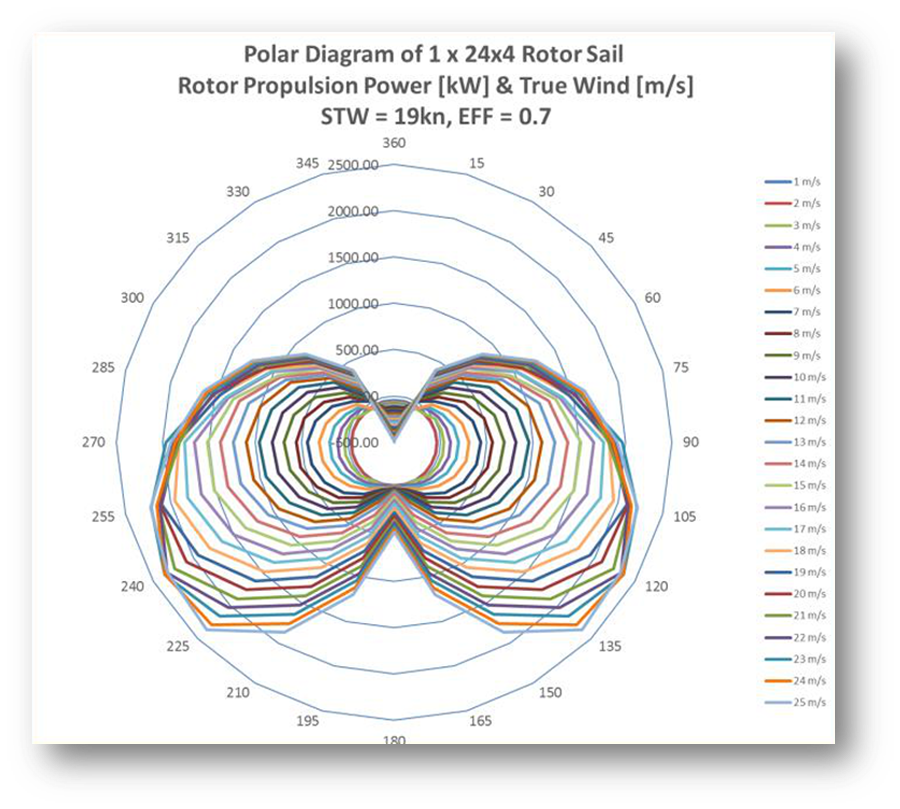
\includegraphics[width=\columnwidth, height=0.65\textheight, keepaspectratio]{Rotor_characteristics.png}
\end{column}
\end{columns}
\end{frame}

%------------------------
\begin{frame}{Vessel and rotor specification}
\begin{columns}
\begin{column}{0.52\textwidth}
\centering
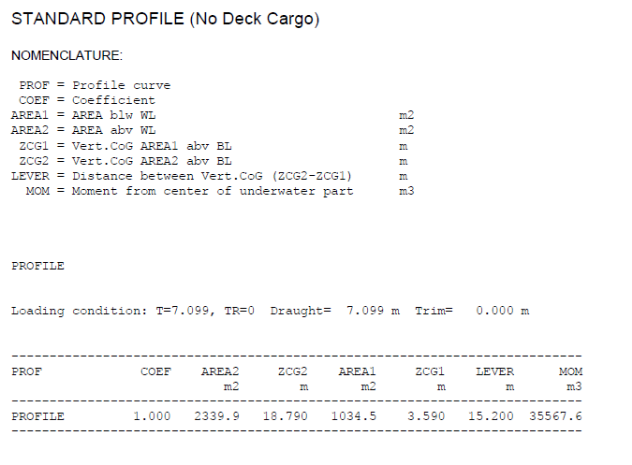
\includegraphics[width=\columnwidth, height=0.65\textheight, keepaspectratio]{Vessel_specification.png}
\end{column}
\begin{column}{0.44\textwidth}
\footnotesize
\textbf{Key parameters used in the analysis}
\begin{itemize}
  \item Design speed: 11.5 kn
  \item Design brake power: 3,500 kW
  \item Resistance model: cubic (power $\propto$ speed$^3$)
  \item SFOC: 195 g/kWh
  \item HFO CO$_2$ factor: 3.114 t CO$_2$/t fuel
  \item Rotor active conditions: $P_\text{rotor}>0$, $H_s \leq 6$ m, $U_\text{wind} \leq 42$ m/s
  \item Power-to-speed conversion: 200 kW $\approx$ 1 kn at operating point
\end{itemize}

\begin{block}{Note}
All scenario values flow from a single set of consistent assumptions applied throughout every extension notebook.
\end{block}
\end{column}
\end{columns}
\end{frame}

%------------------------
\begin{frame}{Data sources and trajectories}
\begin{columns}
\begin{column}{0.52\textwidth}
\centering
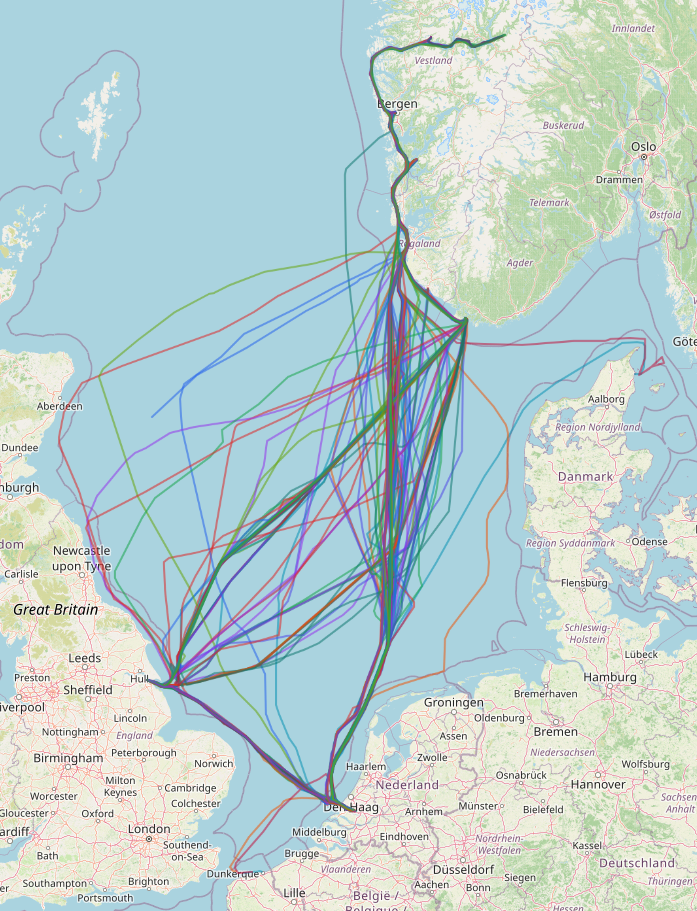
\includegraphics[width=\columnwidth, height=0.56\textheight, keepaspectratio]{all_trajectories_osm.png}
{\small North Sea AIS traces on OpenStreetMap basemap.}
\end{column}
\begin{column}{0.45\textwidth}
\footnotesize
\begin{center}
\begin{tabular}{ll}
\toprule
\textbf{Property} & \textbf{Value} \\
\midrule
Period           & 2023-02-02 to 2026-02-02 \\
Voyages          & 528 \\
Total rows       & 125,160 \\
Training voyages & 422 (88,346 rows) \\
Test voyages     & 106 (35,758 rows) \\
\bottomrule
\end{tabular}
\end{center}
\vspace{0.1cm}
\textbf{Data layers joined per AIS point}
\begin{itemize}
  \item \textbf{ERA5}: 10 m wind components, gusts
  \item \textbf{Copernicus Marine}: significant wave height $H_s$, mean wave direction \& period
  \item \textbf{Copernicus currents}: eastward \& northward current components
\end{itemize}

\begin{block}{Key}
Spatio-temporal interpolation attaches metocean state to each AIS observation.
\end{block}
\end{column}
\end{columns}
\end{frame}

% ============================================================
%  PART 2 - METHODOLOGY
% ============================================================

\sectiondivider{Part II}{Methodology \& Models}{Olga Grigorieva}{Feature engineering $\cdot$ Model hierarchy $\cdot$ Speed prediction results}

%------------------------
\begin{frame}{Feature engineering: leakage-aware design}
\begin{columns}
\begin{column}{0.50\textwidth}
\footnotesize
\textbf{Feature groups}
\begin{itemize}
  \item \textbf{Wind/wave}: true wind speed, $H_s$, wave period, wind$^2$, wave-wind alignment
  \item \textbf{Angle encoding}: $\sin\alpha$, $\cos\alpha$ for relative wind - avoids 0/360 discontinuity
  \item \textbf{Apparent wind}: speed \& angle as experienced by the moving vessel
  \item \textbf{Currents}: magnitude, direction, along-course and cross-course components
  \item \textbf{Nowcast lags}: SOG$_{t-1}$, SOG$_{t-2}$, rolling mean$_3$ - grouped by voyage
  \item \textbf{Interactions}: wind-angle, wave-wind, current-course nonlinear terms
\end{itemize}
\end{column}
\begin{column}{0.46\textwidth}
\footnotesize
\textbf{Leakage controls}
\begin{itemize}
  \item Lag features never use the \textit{current} target row
  \item Rolling windows reset at voyage boundaries - no cross-voyage borrowing
  \item Rotor variables are \textbf{not} training features; applied post-prediction only
  \item Chronological voyage split: test set is later in time than training set
\end{itemize}

\begin{block}{Key takeaway}
Weather-only and lagged nowcast models use \emph{disjoint} feature sets - explanatory and predictive questions are kept separate.
\end{block}
\end{column}
\end{columns}
\end{frame}

%------------------------
\begin{frame}{Model hierarchy and rotor scenario methodology}
\begin{columns}
\begin{column}{0.50\textwidth}
\footnotesize
\textbf{Four model levels for SOG prediction}
\begin{center}
\begin{tabular}{lp{4.4cm}}
\toprule
\textbf{Model} & \textbf{Description} \\
\midrule
B1 & Constant mean training speed \\
B2 & Linear: wind speed, $H_s$, $\sin\alpha$, $\cos\alpha$ \\
M1 & XGBoost, weather-only features \\
M2 & XGBoost, weather + lagged SOG (nowcast) \\
\bottomrule
\end{tabular}
\end{center}
XGBoost: 300 trees, depth 6, lr 0.05, 80\% row/col subsampling.

\vspace{0.2cm}
\textbf{95\% prediction interval} (M2 quantile regression):\\
mean width 3.161 kn, empirical coverage 96.5\%.
\end{column}
\begin{column}{0.46\textwidth}
\footnotesize
\textbf{Rotor scenario (post-prediction layer)}
\[
\Delta\text{SOG} = \frac{P_\text{rotor}}{200\,\text{kW/kn}}
\]
Active when $P_\text{rotor}>0$, $H_s \leq 6$ m, $U \leq 42$ m/s.

$P_\text{rotor}$ read from the supplied polar-response table (wind speed $\times$ relative angle).

\vspace{0.1cm}
\textbf{Weather window criterion}
\[
\text{SOG} \geq 10\,\text{kn} \quad\text{and}\quad H_s \leq 3\,\text{m}
\]
Contiguous observations satisfying both = one window.

\begin{block}{Design choice}
Rotor is a scenario overlay, not a training feature - baseline and rotor-assisted results are directly comparable.
\end{block}
\end{column}
\end{columns}
\end{frame}

% ============================================================
%  PART 3 - MODEL RESULTS
% ============================================================

%------------------------
\begin{frame}{Model results: held-out test performance}
\begin{columns}
\begin{column}{0.48\textwidth}
{\scriptsize\setlength\tabcolsep{3.5pt}
\begin{center}
\begin{tabular}{lrrrr}
\toprule
\textbf{Model} & \textbf{MAE} & \textbf{RMSE} & \textbf{$R^2$} & \textbf{$\pm$1kn} \\
\midrule
B1: Constant     & 1.388 & 1.893 & -0.002 & 49.3\% \\
B2: Linear       & 1.377 & 1.860 & 0.034  & 49.5\% \\
M1: XGB weather  & 1.468 & 1.883 & 0.010  & 41.7\% \\
\textbf{M2: Nowcast} & \textbf{0.406} & \textbf{0.758} & \textbf{0.839} & \textbf{91.7\%} \\
\bottomrule
\end{tabular}
\end{center}}

{\scriptsize All errors in knots. Voyage split: 106 test voyages.}

\vspace{0.15cm}
\footnotesize\textbf{Interpretation}
\begin{itemize}\footnotesize
  \item B1/B2 nearly identical - wind/wave has limited linear signal.
  \item M1 does not beat linear baseline - weather-only generalisation is hard.
  \item M2 works: recent SOG encodes engine setting, cargo, operational state.
\end{itemize}
\end{column}
\begin{column}{0.49\textwidth}
\centering
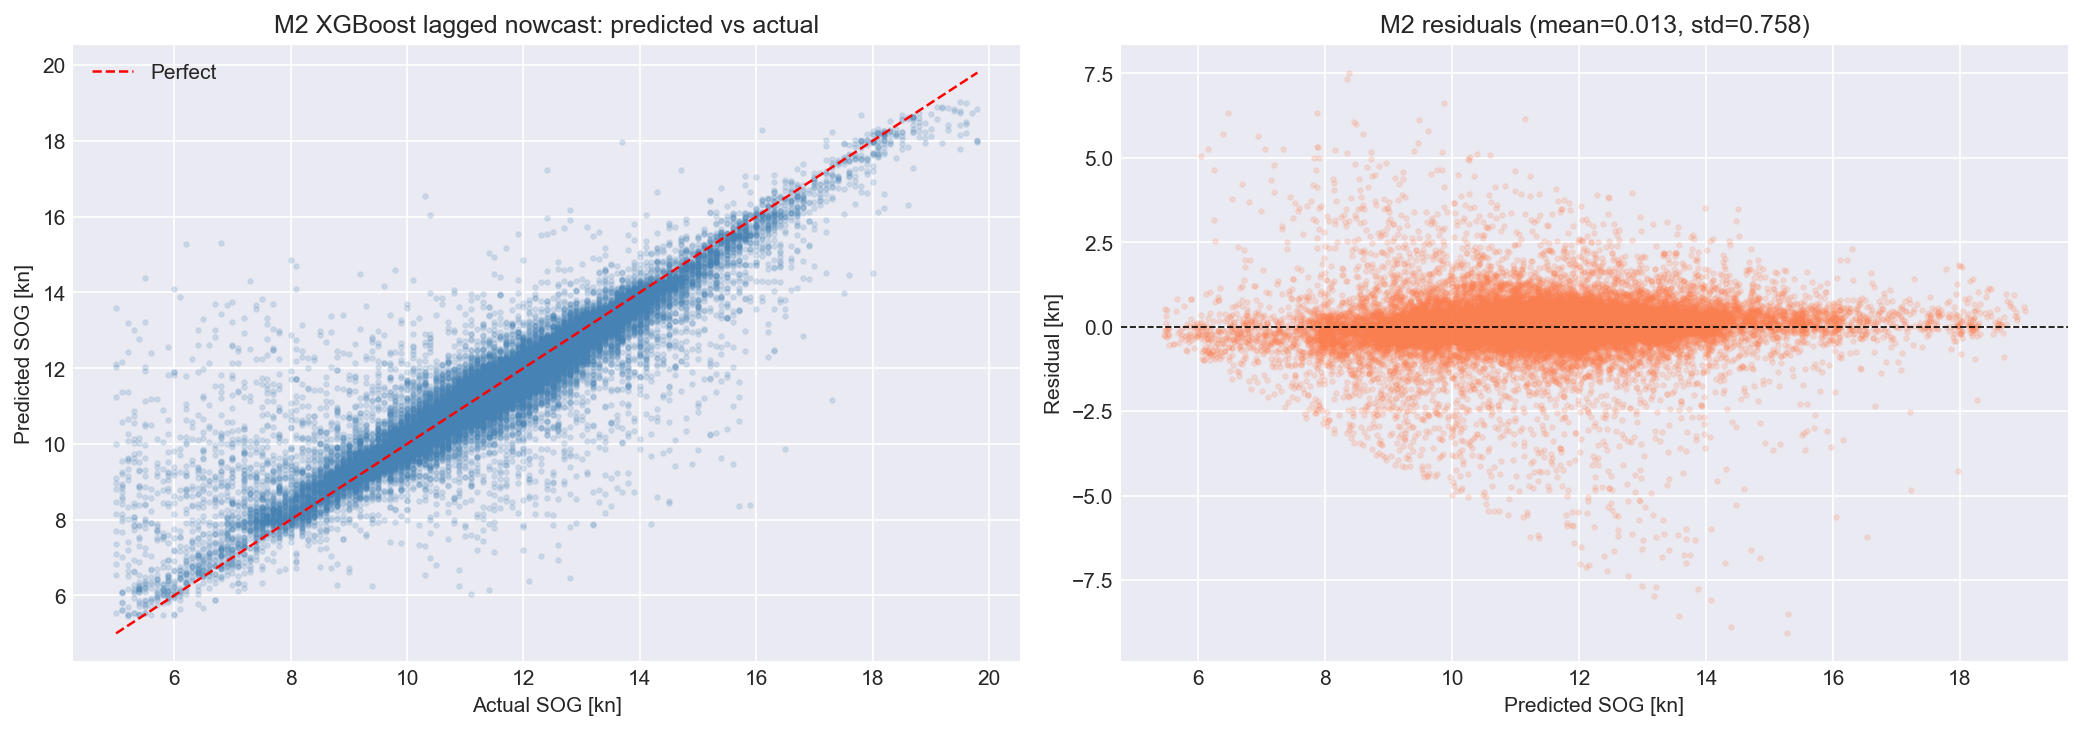
\includegraphics[width=\columnwidth, height=0.58\textheight, keepaspectratio]{predicted_vs_actual.png}
{\small M2 predicted vs.\ actual SOG (test set).}
\end{column}
\end{columns}
\end{frame}

%------------------------
\begin{frame}{Feature importance and prediction intervals}
\begin{columns}
\begin{column}{0.56\textwidth}
\centering
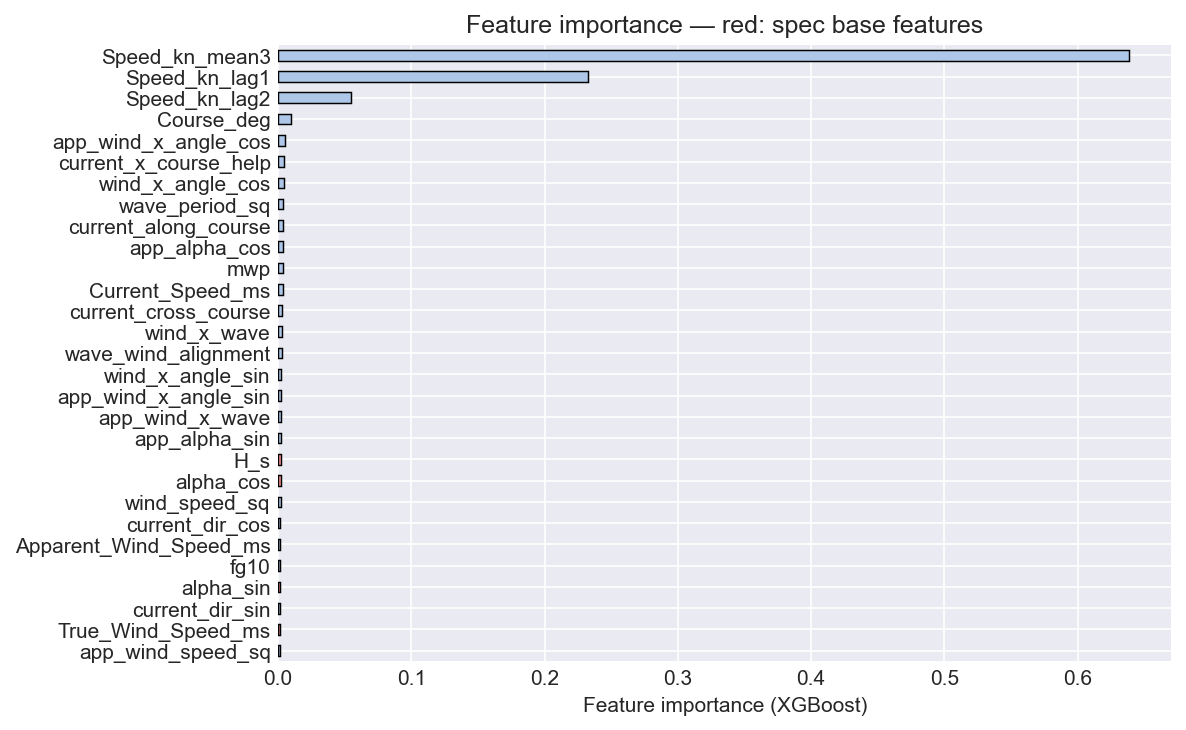
\includegraphics[width=\columnwidth, height=0.52\textheight, keepaspectratio]{feature_importance.png}
{\small Weather-only (left) and lagged nowcast (right) XGBoost importances.}
\end{column}
\begin{column}{0.41\textwidth}
\footnotesize
\textbf{Weather-only (M1)}: course and current interaction terms rank highest. Wind/wave present but not dominant - missing operational variables limit explanatory power.

\vspace{0.15cm}
\textbf{Nowcast (M2)}: lagged SOG dominates - recent speed summarises engine setting, route, and loading. Apparent wind angle enters top features; weather secondary.

\begin{block}{Key takeaway}
Speed persistence is the main signal; weather effects need additional operational variables to isolate cleanly.
\end{block}
\end{column}
\end{columns}
\end{frame}

% ============================================================
%  PART 3 - ROTOR PERFORMANCE
% ============================================================

\sectiondivider{Part III}{Rotor Performance}{Elen Mouradian}{Speed uplift $\cdot$ Weather windows $\cdot$ Gain surface $\cdot$ Energy \& CO\textsubscript{2}}

%------------------------
\begin{frame}{Rotor scenario: speed uplift and weather-window impact}
\begin{columns}
\begin{column}{0.54\textwidth}
\centering
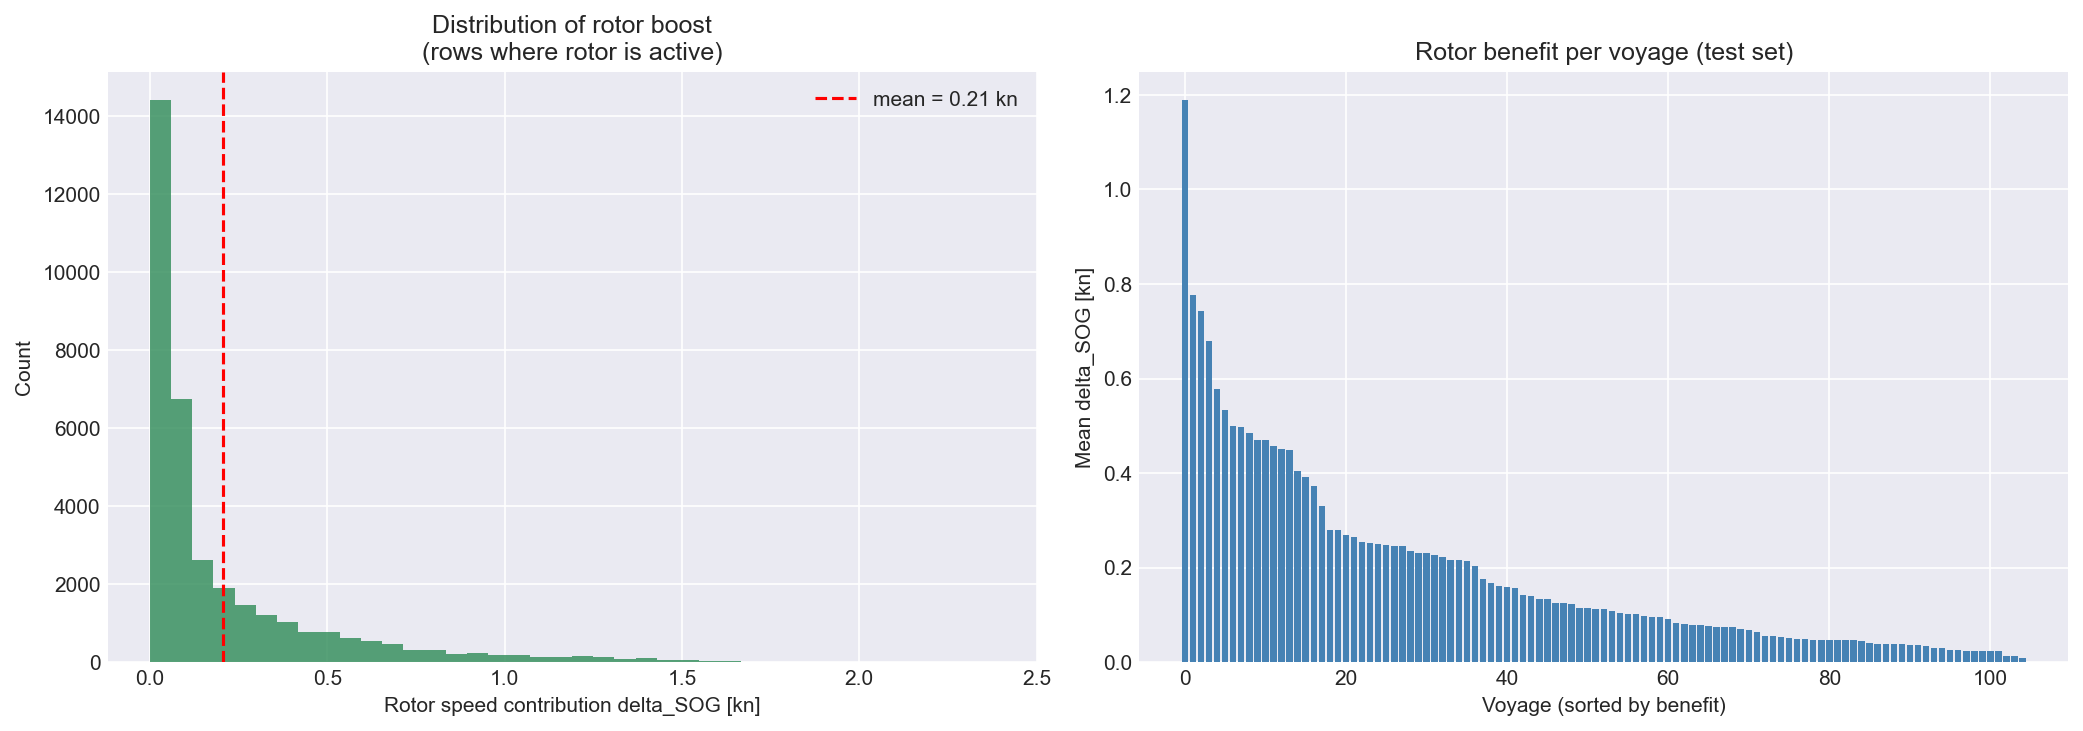
\includegraphics[width=\columnwidth, height=0.54\textheight, keepaspectratio]{rotor_scenario.png}
{\small Rotor power distribution and per-voyage mean speed contribution.}
\end{column}
\begin{column}{0.43\textwidth}
\footnotesize
\textbf{Test-set rotor summary}
\begin{center}
\begin{tabular}{ll}
\toprule
Active share & 98.1\% \\
Mean active power & 41.2 kW \\
Mean active $\Delta$SOG & 0.206 kn \\
Overall mean $\Delta$SOG & 0.202 kn \\
\bottomrule
\end{tabular}
\end{center}

\textbf{Weather-window impact}
\begin{center}
\begin{tabular}{lrr}
\toprule
 & \textbf{Windows} & \textbf{Coverage} \\
\midrule
Baseline & 866 & 76.0\% \\
+Rotor & 808 & 77.5\% \\
$\Delta$ & -58 & +1.5 pp \\
\bottomrule
\end{tabular}
\end{center}

\begin{block}{Key takeaway}
Fewer but longer windows: rotor merges marginal periods. Coverage +529 test points inside windows.
\end{block}
\end{column}
\end{columns}
\end{frame}

%------------------------
\begin{frame}{Rotor gain surface: where does it help?}
\centering
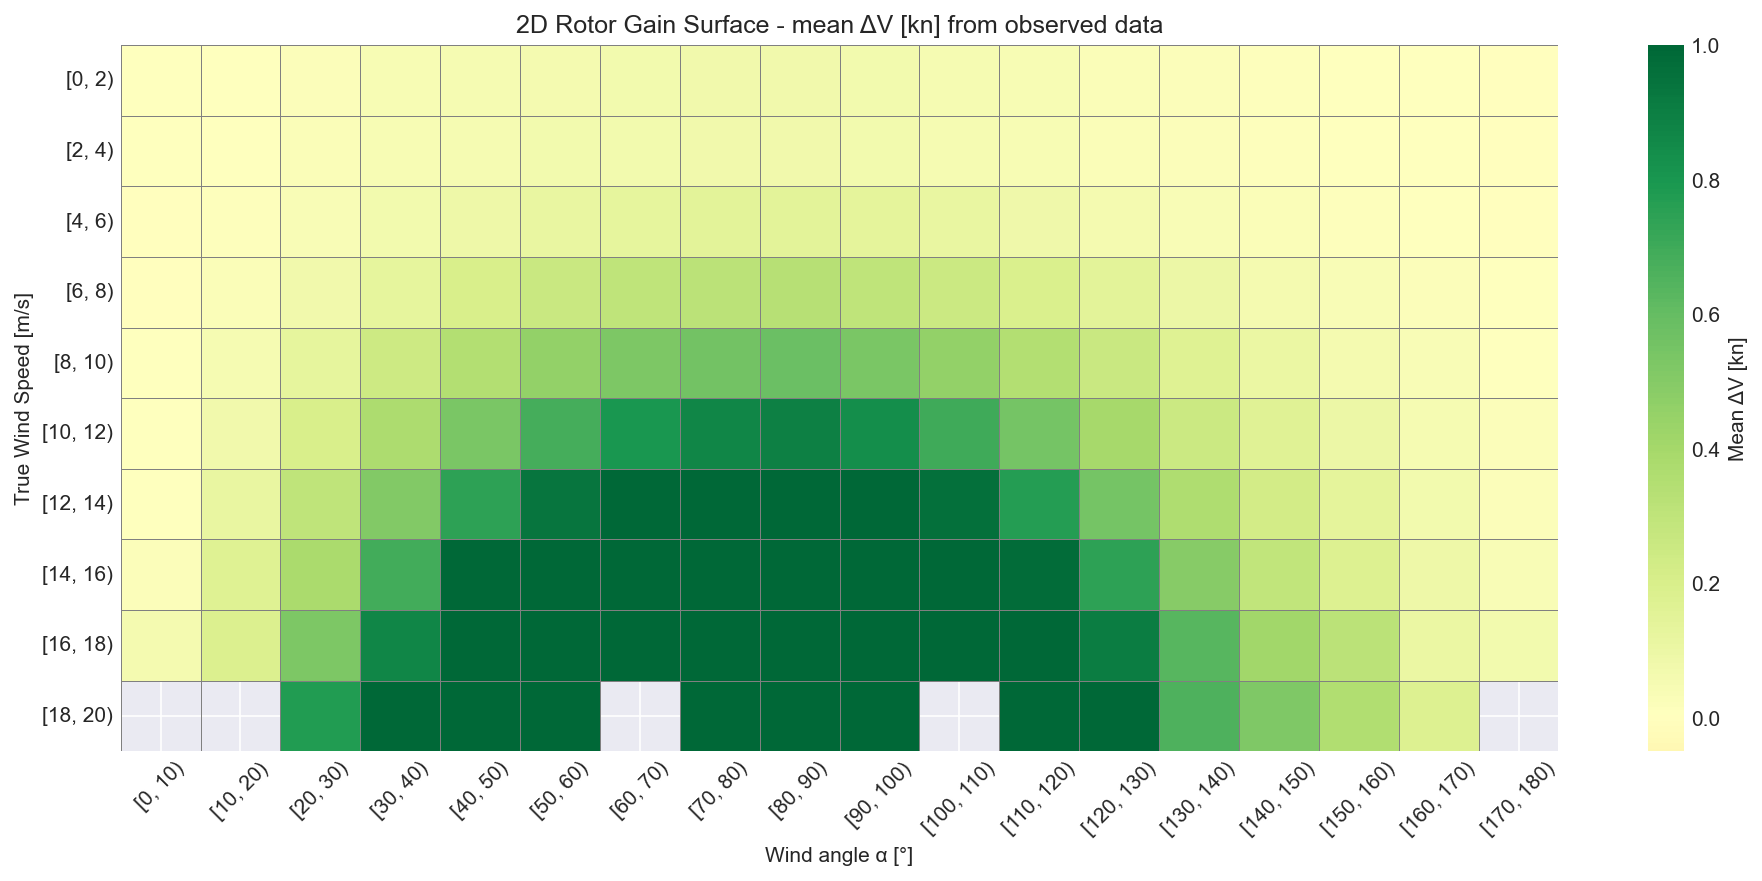
\includegraphics[width=0.95\textwidth, height=0.56\textheight, keepaspectratio]{rotor_gain_surface.png}

{\small Gain concentrated at beam/quartering angles (50-130$^\circ$) above 8 m/s. Headwind/tailwind sectors poor. Sea state acts as a gate, not a gain driver.}

\begin{block}{Key takeaway}
Rotor benefit is directional and speed-dependent - ``good wind'' is not enough; the angle must be right.
\end{block}
\end{frame}

% ============================================================
%  PART 5 - EXTENSIONS
% ============================================================

%------------------------
\begin{frame}{Extension 1: Energy, fuel, and CO$_2$ impact}
\begin{columns}
\begin{column}{0.55\textwidth}
\centering
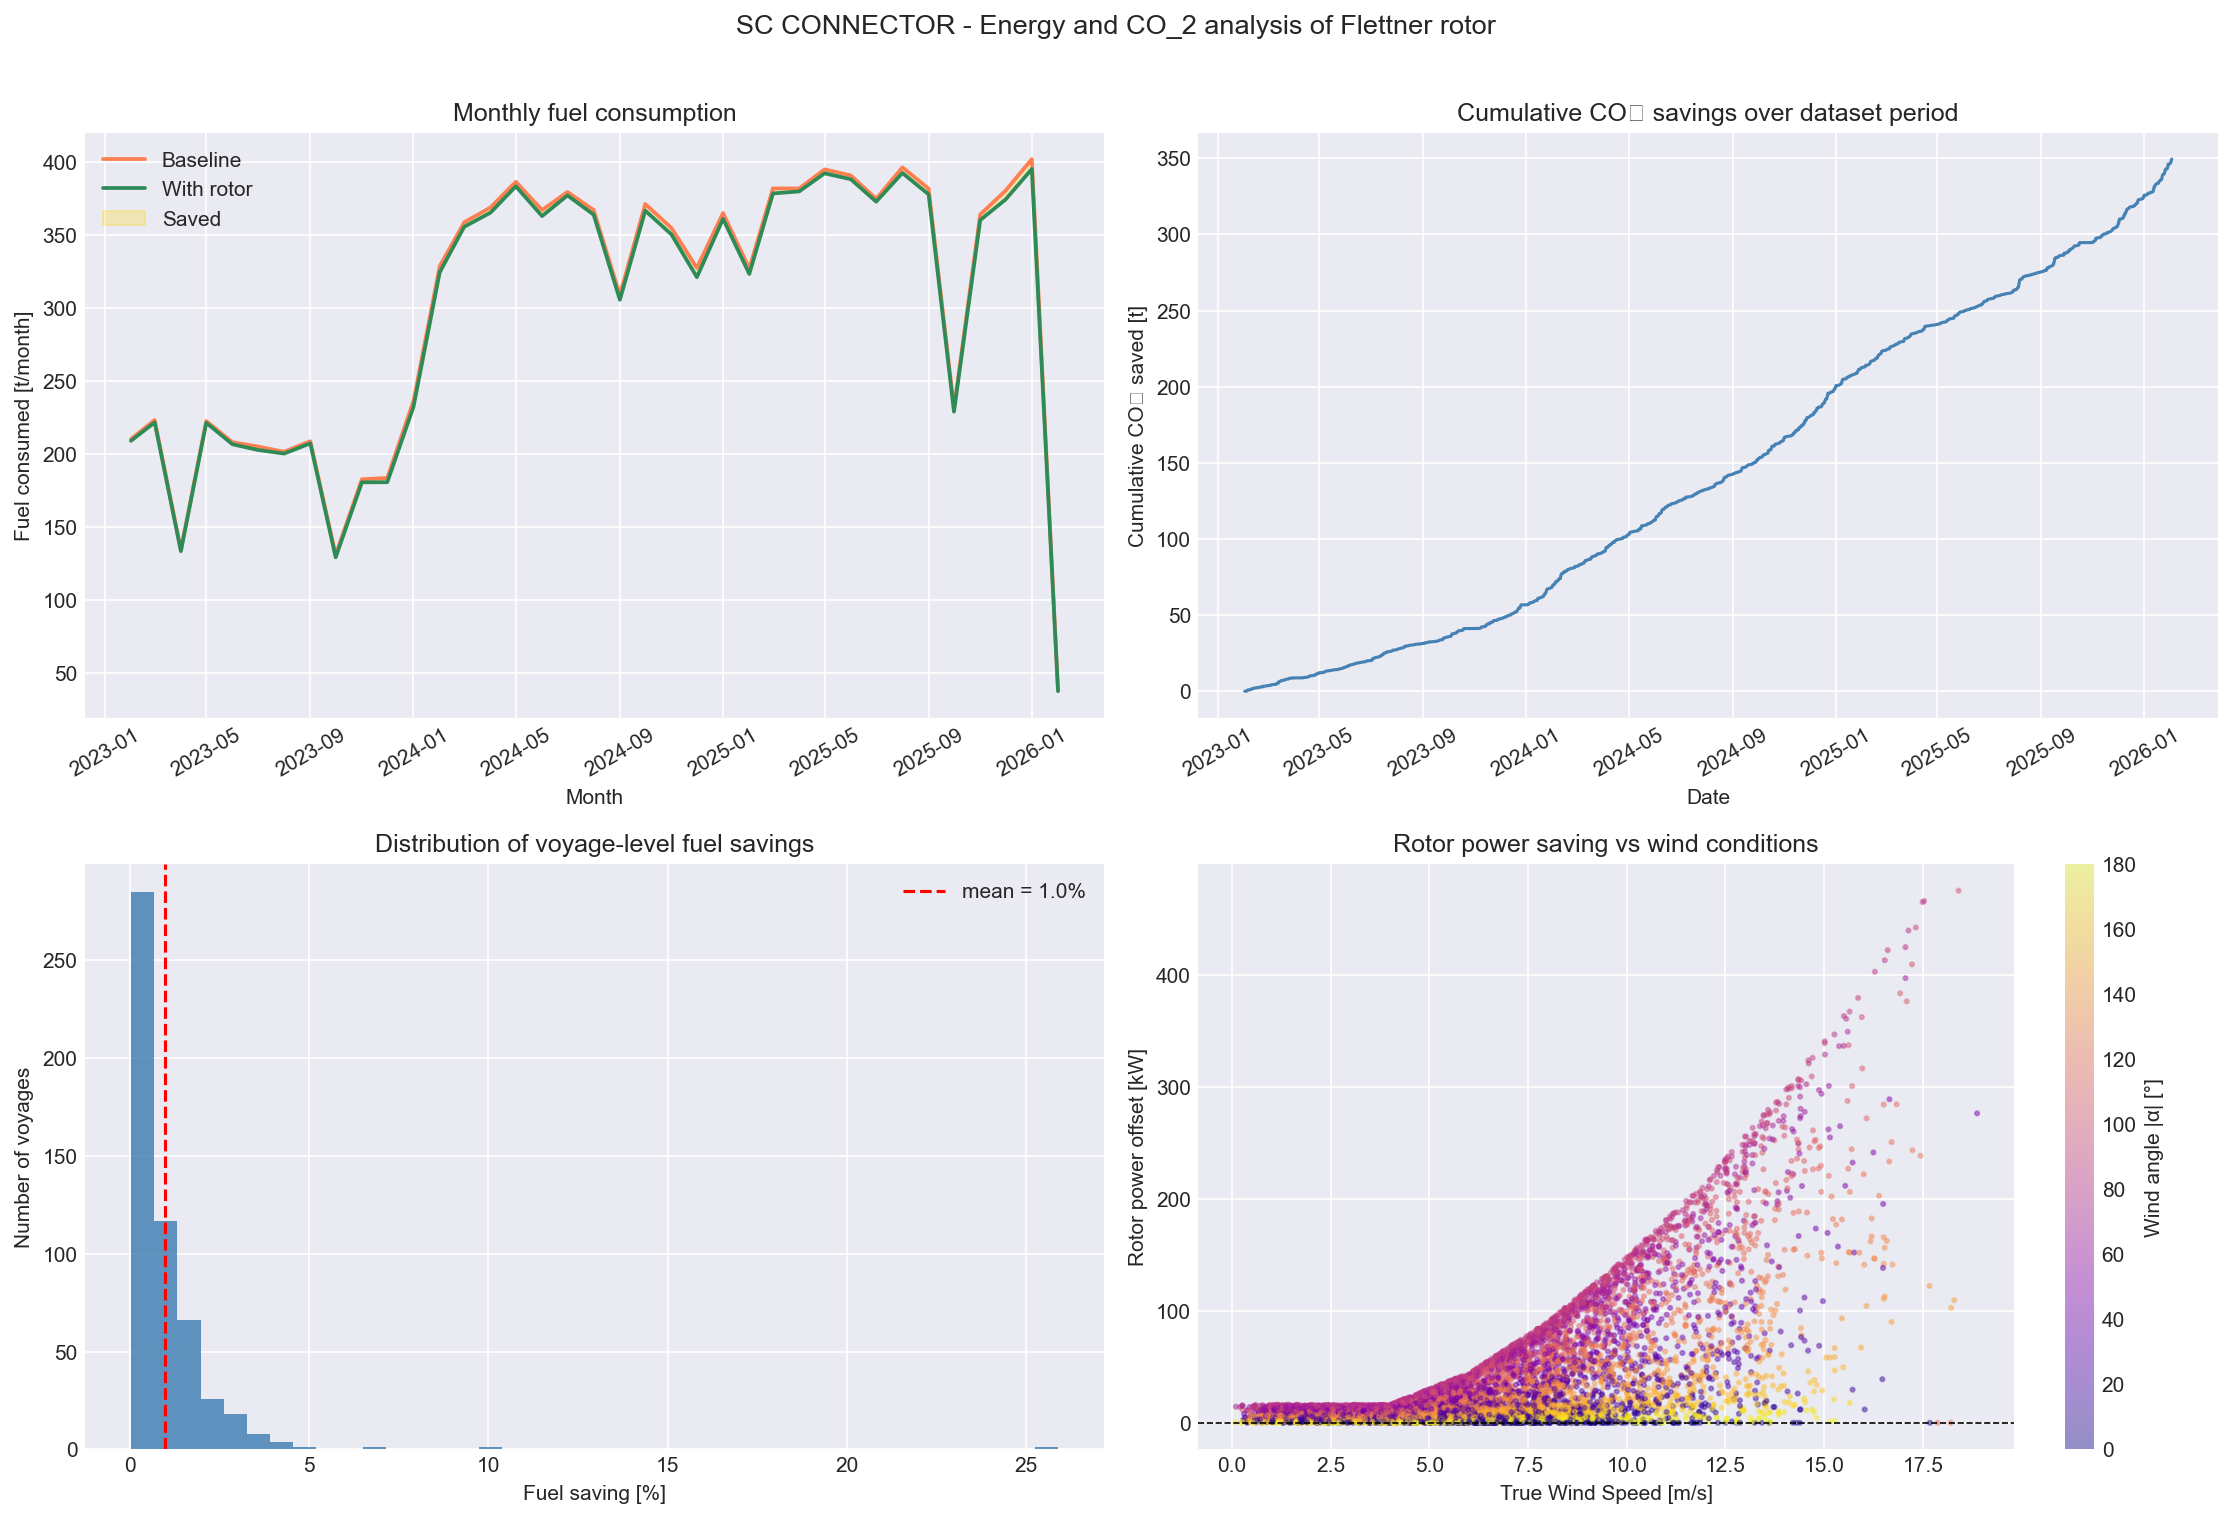
\includegraphics[width=\columnwidth, height=0.55\textheight, keepaspectratio]{energy_fuel_co2.png}
{\small Fuel and CO$_2$ impact from the rotor energy model.}
\end{column}
\begin{column}{0.42\textwidth}
\footnotesize
\textbf{Three-year dataset summary}
\begin{center}
\begin{tabular}{ll}
\toprule
Rotor active share & 97.6\% \\
Fuel baseline & 11,067 t \\
Fuel w/ rotor & 10,954 t \\
Fuel saved & 112.2 t (1.01\%) \\
CO$_2$ saved & 349.4 t (1.01\%) \\
\bottomrule
\end{tabular}
\end{center}

\textbf{Annualised estimate}
\begin{itemize}
  \item 37.4 t fuel saved/year
  \item 116.4 t CO$_2$ avoided/year
  \item CII: 53.75 $\to$ 53.20 g CO$_2$/(t nm)
\end{itemize}

\begin{block}{Note}
Cubic resistance model; scenario estimate, not certified trial. Order of magnitude is the robust finding.
\end{block}
\end{column}
\end{columns}
\end{frame}

% ============================================================
%  PART 4 - ROUTE INTELLIGENCE
% ============================================================

\sectiondivider{Part IV}{Route Intelligence}{Bartosz Maj}{Route segmentation $\cdot$ Dijkstra optimisation $\cdot$ High-gain detection}

%------------------------
\begin{frame}{Extension 2: Route segmentation by heading regime}
\begin{columns}
\begin{column}{0.54\textwidth}
\centering
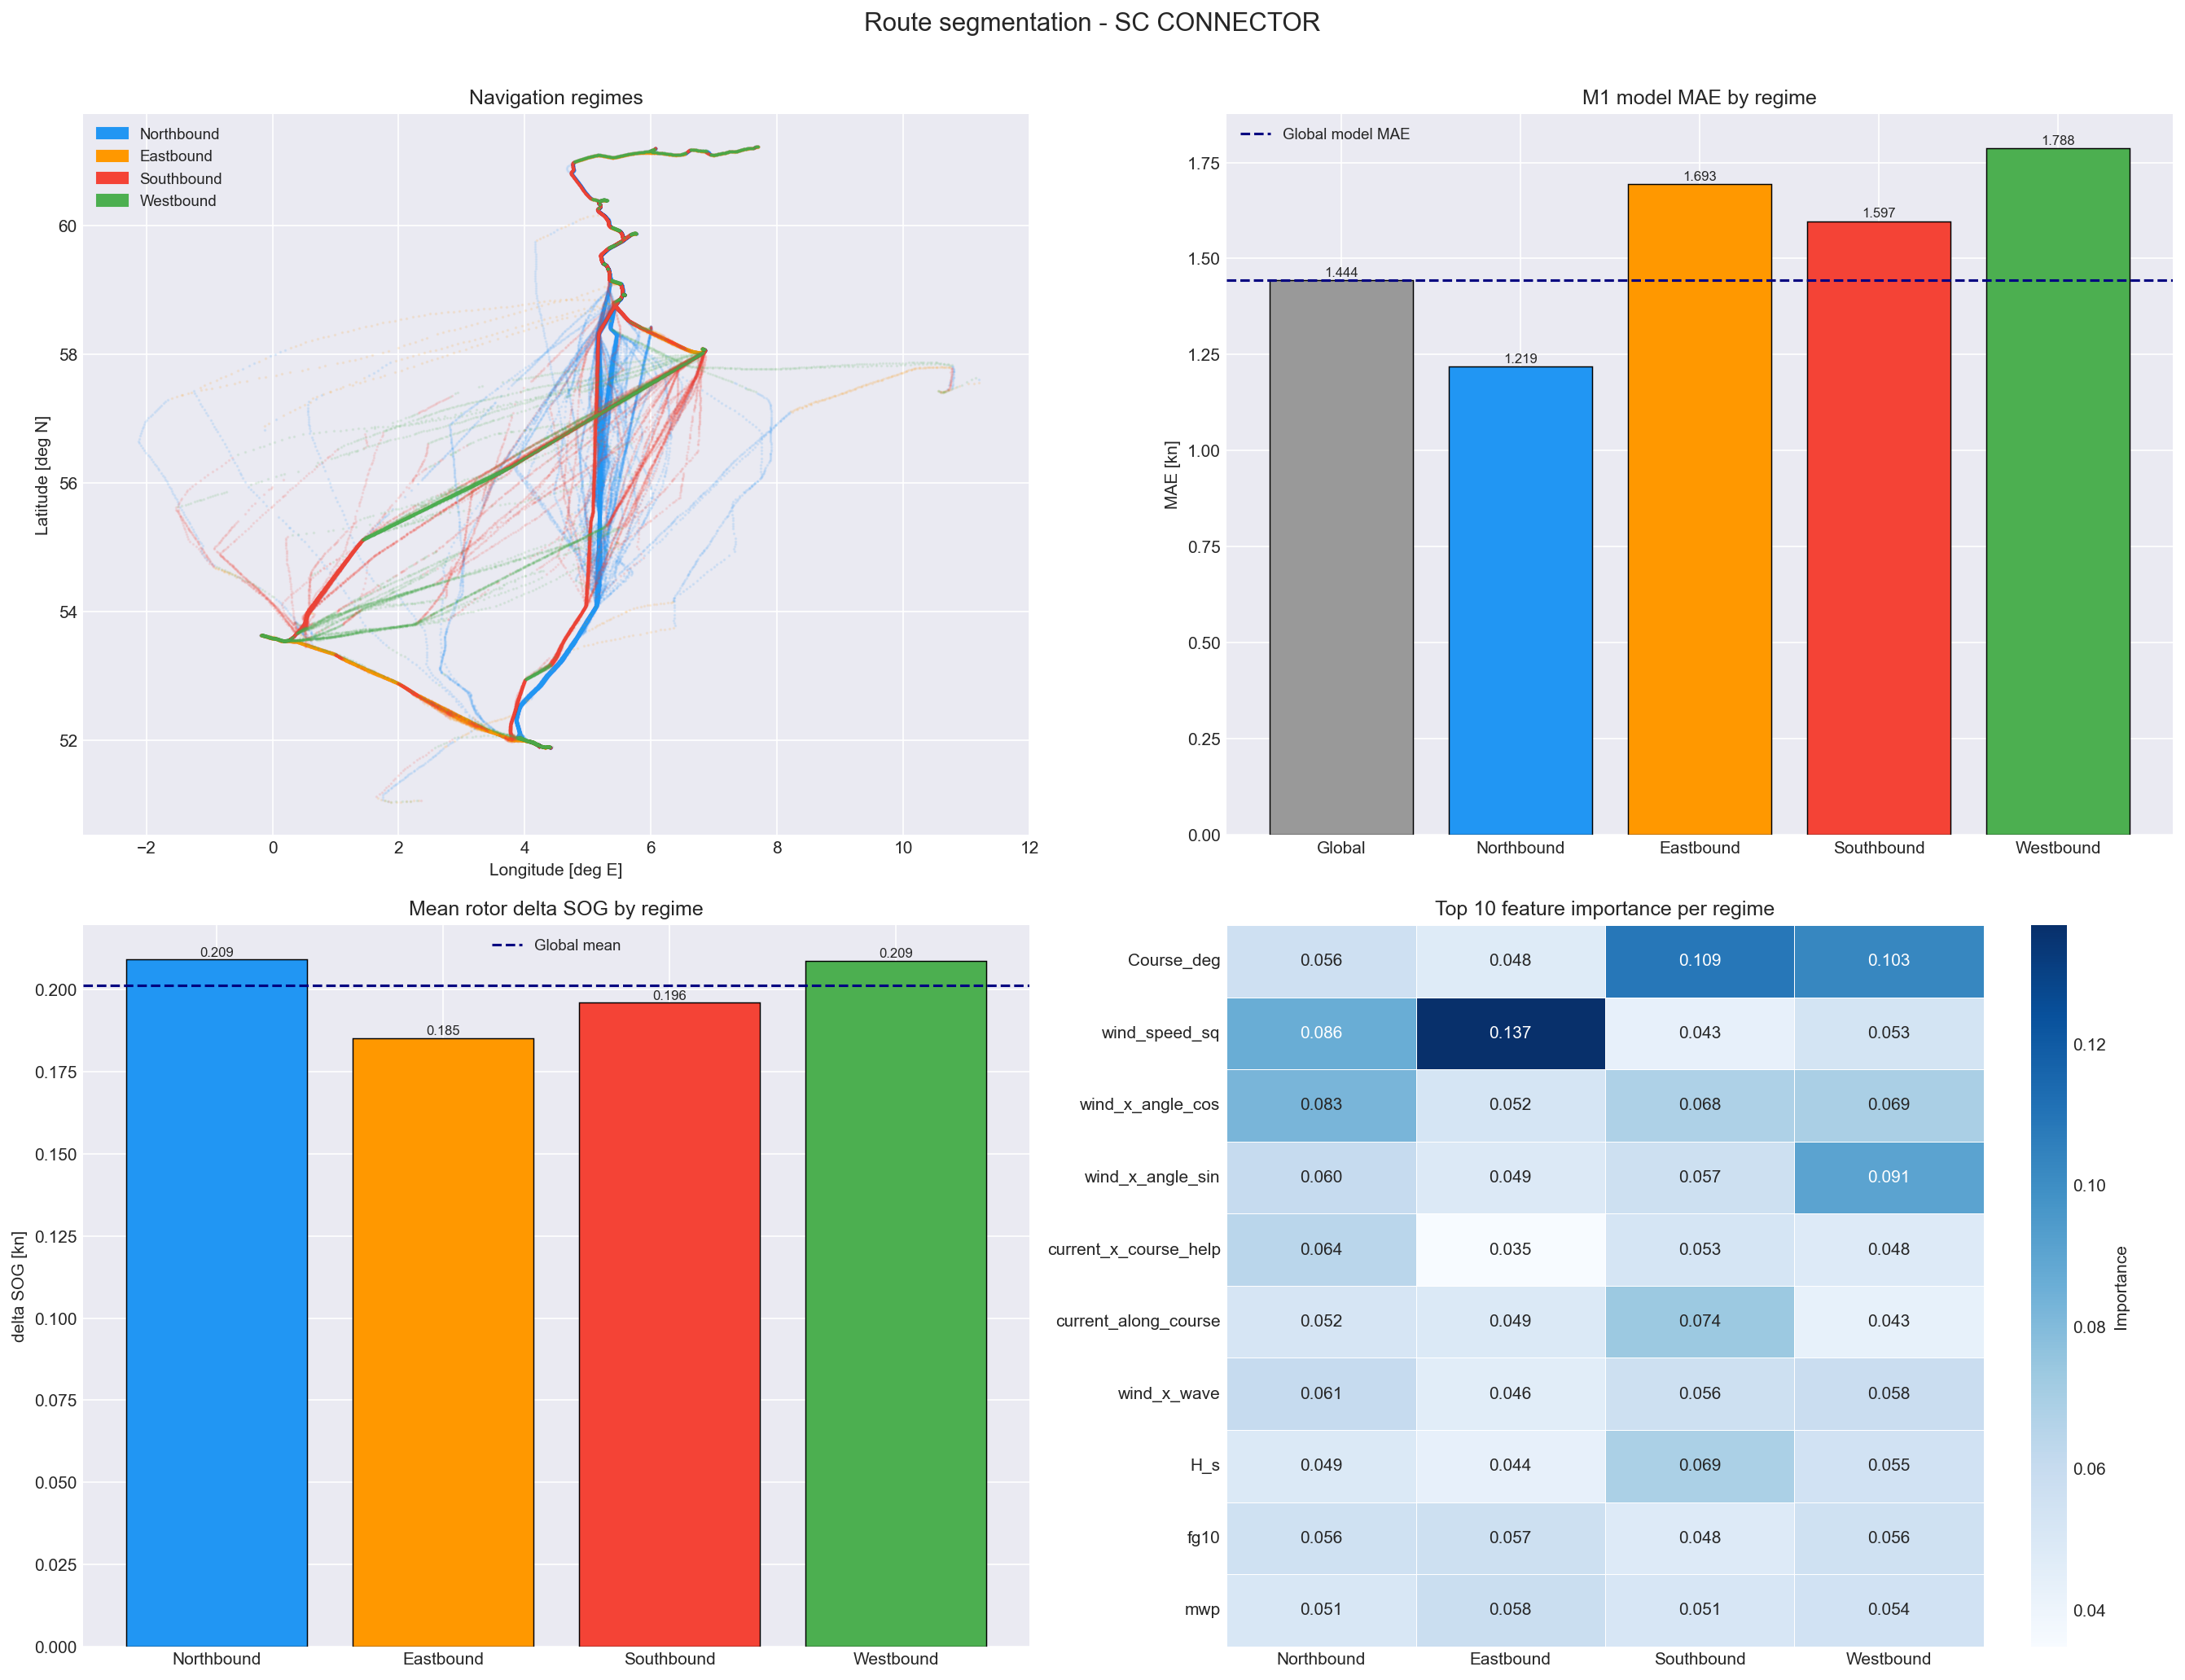
\includegraphics[width=\columnwidth, height=0.55\textheight, keepaspectratio]{route_segmentation.png}
{\small Route segmentation into N/E/S/W heading regimes.}
\end{column}
\begin{column}{0.43\textwidth}
\footnotesize
\textbf{Regime summary (full dataset)}
\begin{center}
\begin{tabular}{lrr}
\toprule
\textbf{Regime} & \textbf{Mean SOG} & \textbf{Mean $\Delta$SOG} \\
\midrule
Northbound & 12.05 kn & 0.209 kn \\
Eastbound  & 12.34 kn & 0.185 kn \\
Southbound & 10.95 kn & 0.196 kn \\
Westbound  & 10.58 kn & 0.209 kn \\
\bottomrule
\end{tabular}
\end{center}

\textbf{Weather-window coverage change}
\begin{itemize}
  \item Westbound: 85.1\% $\to$ \textbf{90.1\%} (largest gain)
  \item Southbound: 82.3\% $\to$ 84.5\%
  \item N/E already at high baseline - smaller delta
\end{itemize}

\begin{block}{Key takeaway}
Westbound legs benefit most - same vessel, different heading geometry creates different rotor opportunity.
\end{block}
\end{column}
\end{columns}
\end{frame}

%------------------------
\begin{frame}{Extension 3: Route optimisation - Dijkstra proof of concept}
\begin{columns}
\begin{column}{0.54\textwidth}
\centering
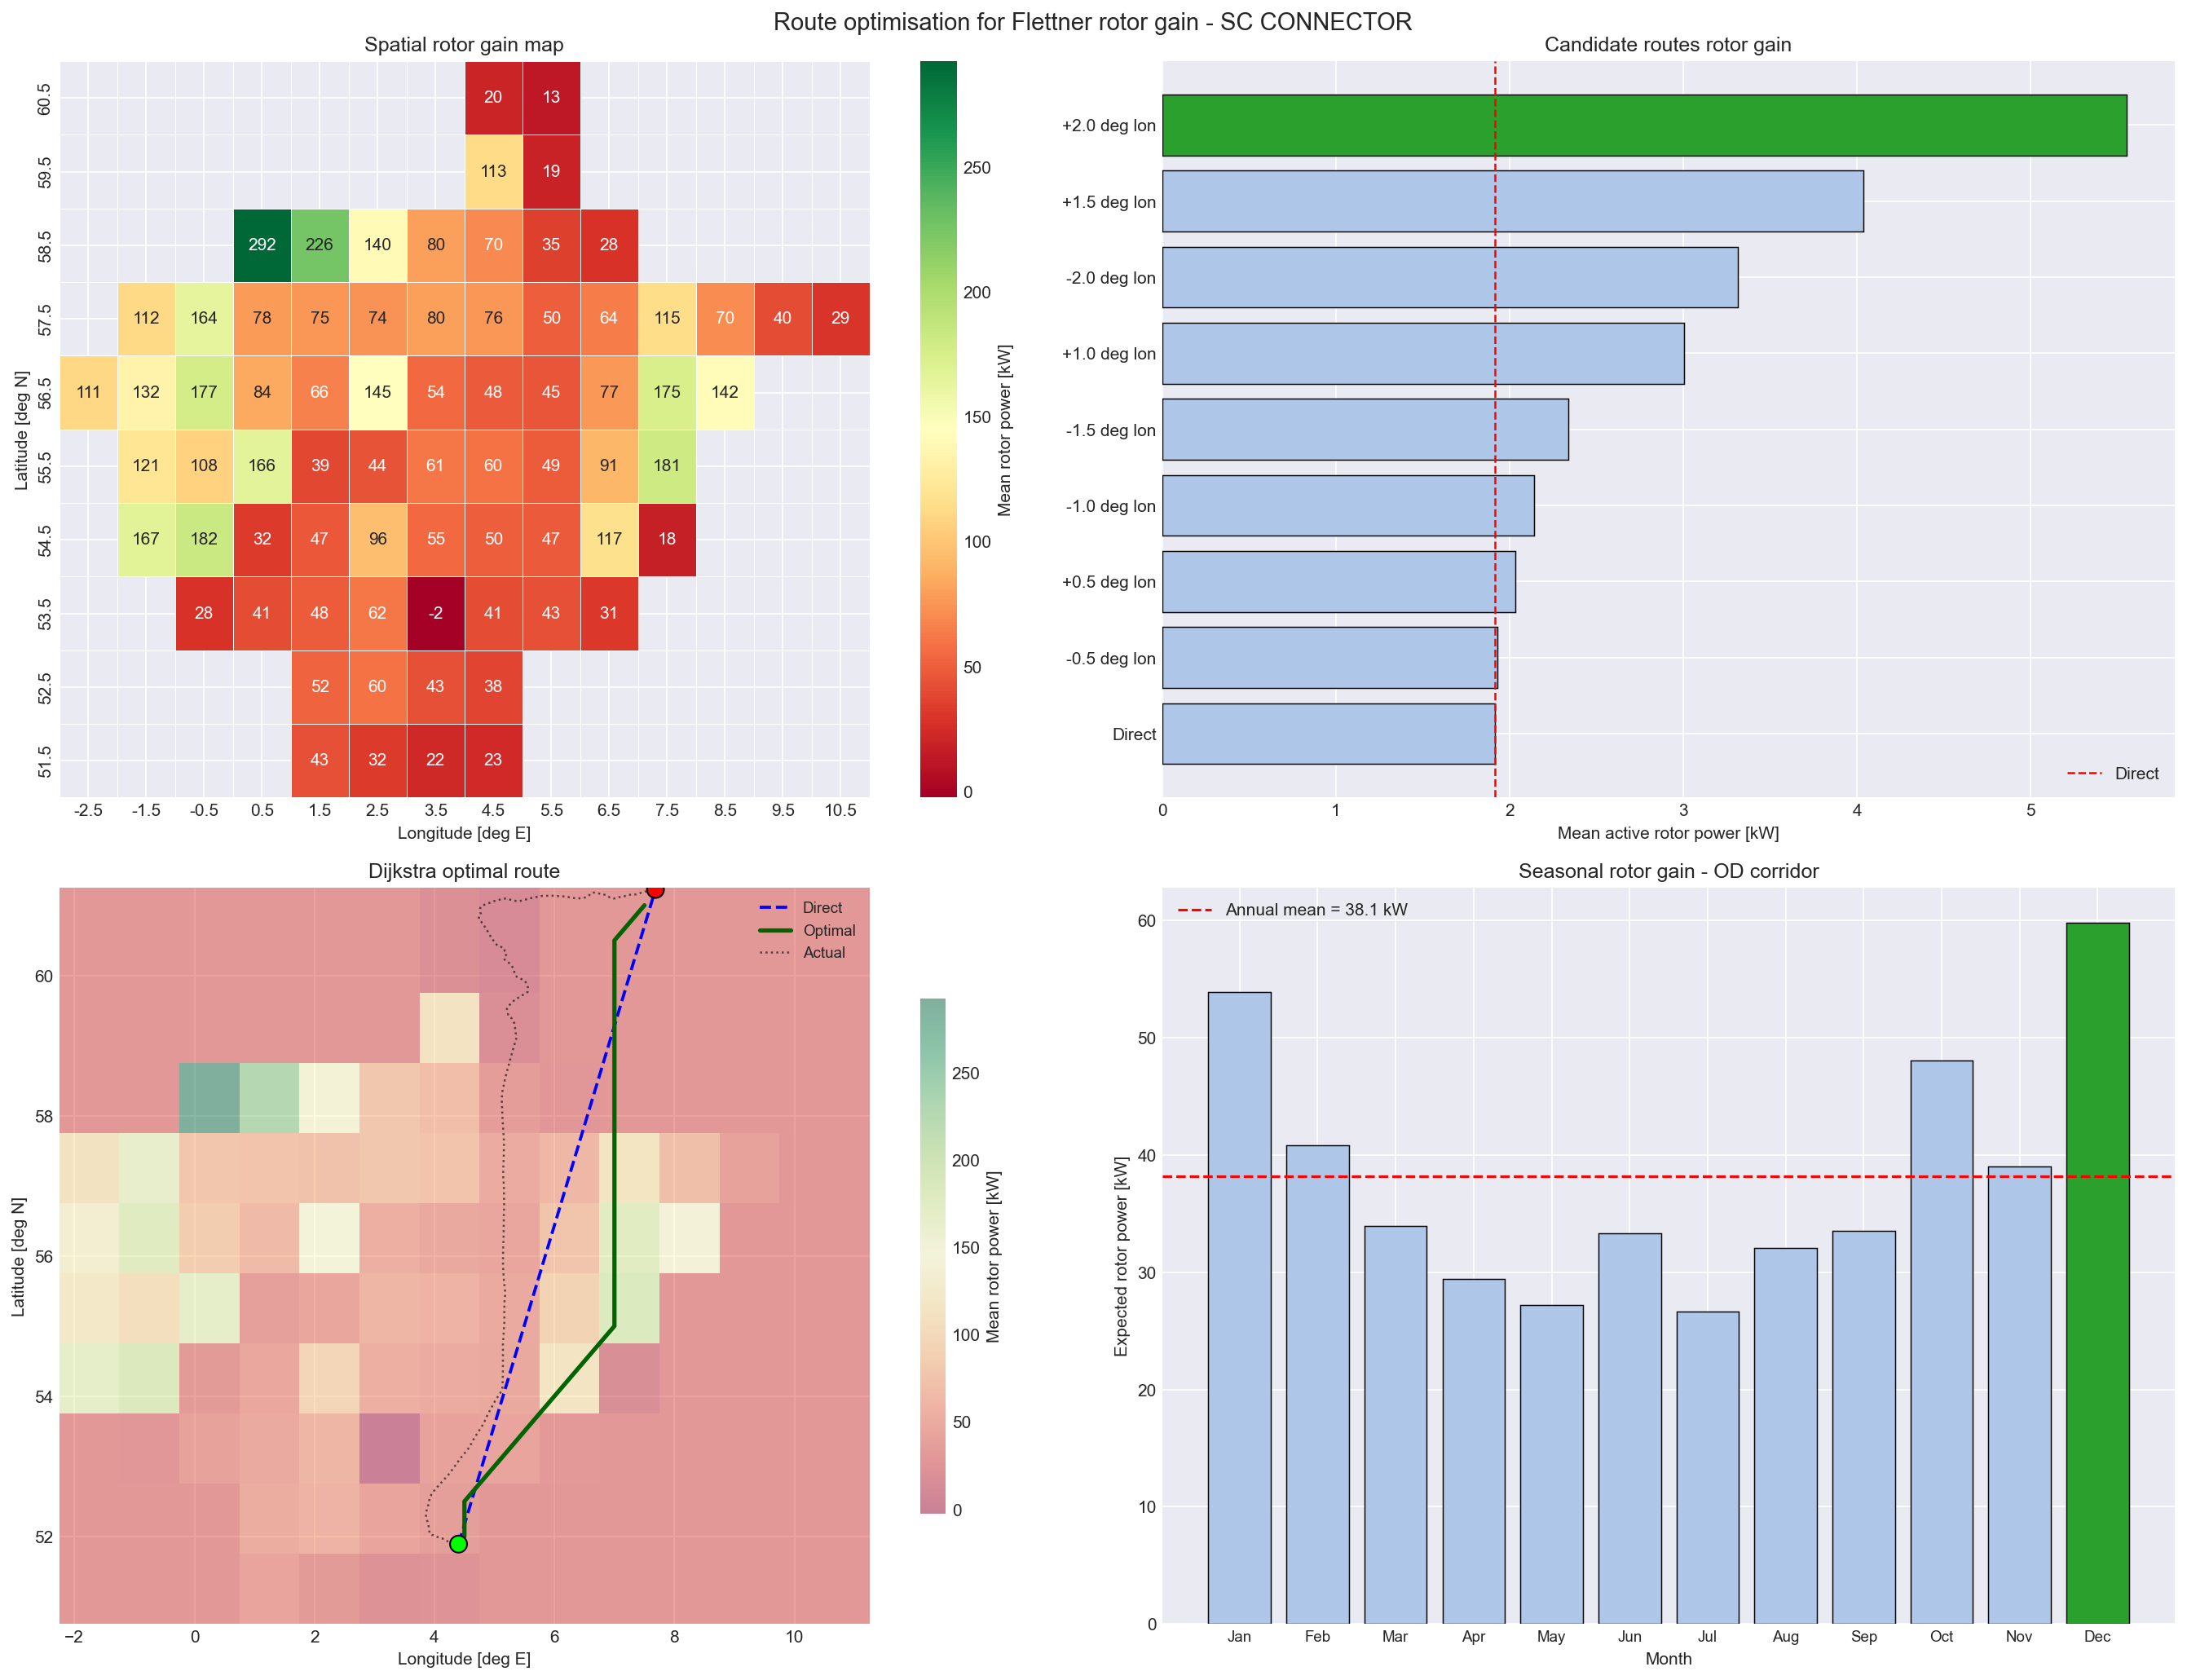
\includegraphics[width=\columnwidth, height=0.55\textheight, keepaspectratio]{route_optimization.png}
{\small Dijkstra grid-search routing for rotor-gain optimisation (Voyage 456).}
\end{column}
\begin{column}{0.43\textwidth}
\footnotesize
\textbf{Voyage 456 result} (Rotterdam $\to$ W. Norway)

\begin{center}
\begin{tabular}{lrr}
\toprule
 & \textbf{Direct} & \textbf{Optimal} \\
\midrule
Distance & 571 nm & 568 nm \\
Mean power & 1.9 kW & 7.5 kW \\
$\Delta$SOG & 0.010 kn & 0.037 kn \\
Gain & \multicolumn{2}{c}{+288\% relative} \\
\bottomrule
\end{tabular}
\end{center}

\textbf{Seasonal best months}: December (59.8 kW avg) vs.\ July (26.6 kW avg)

\begin{block}{Note}
Proof of method: grid is coarse, built from historical fields. Production use needs forecast fields, land mask, traffic separation, safety rules.
\end{block}
\end{column}
\end{columns}
\end{frame}

%------------------------
\begin{frame}{Extension 4: High-gain moment detection}
\begin{columns}
\begin{column}{0.54\textwidth}
\centering
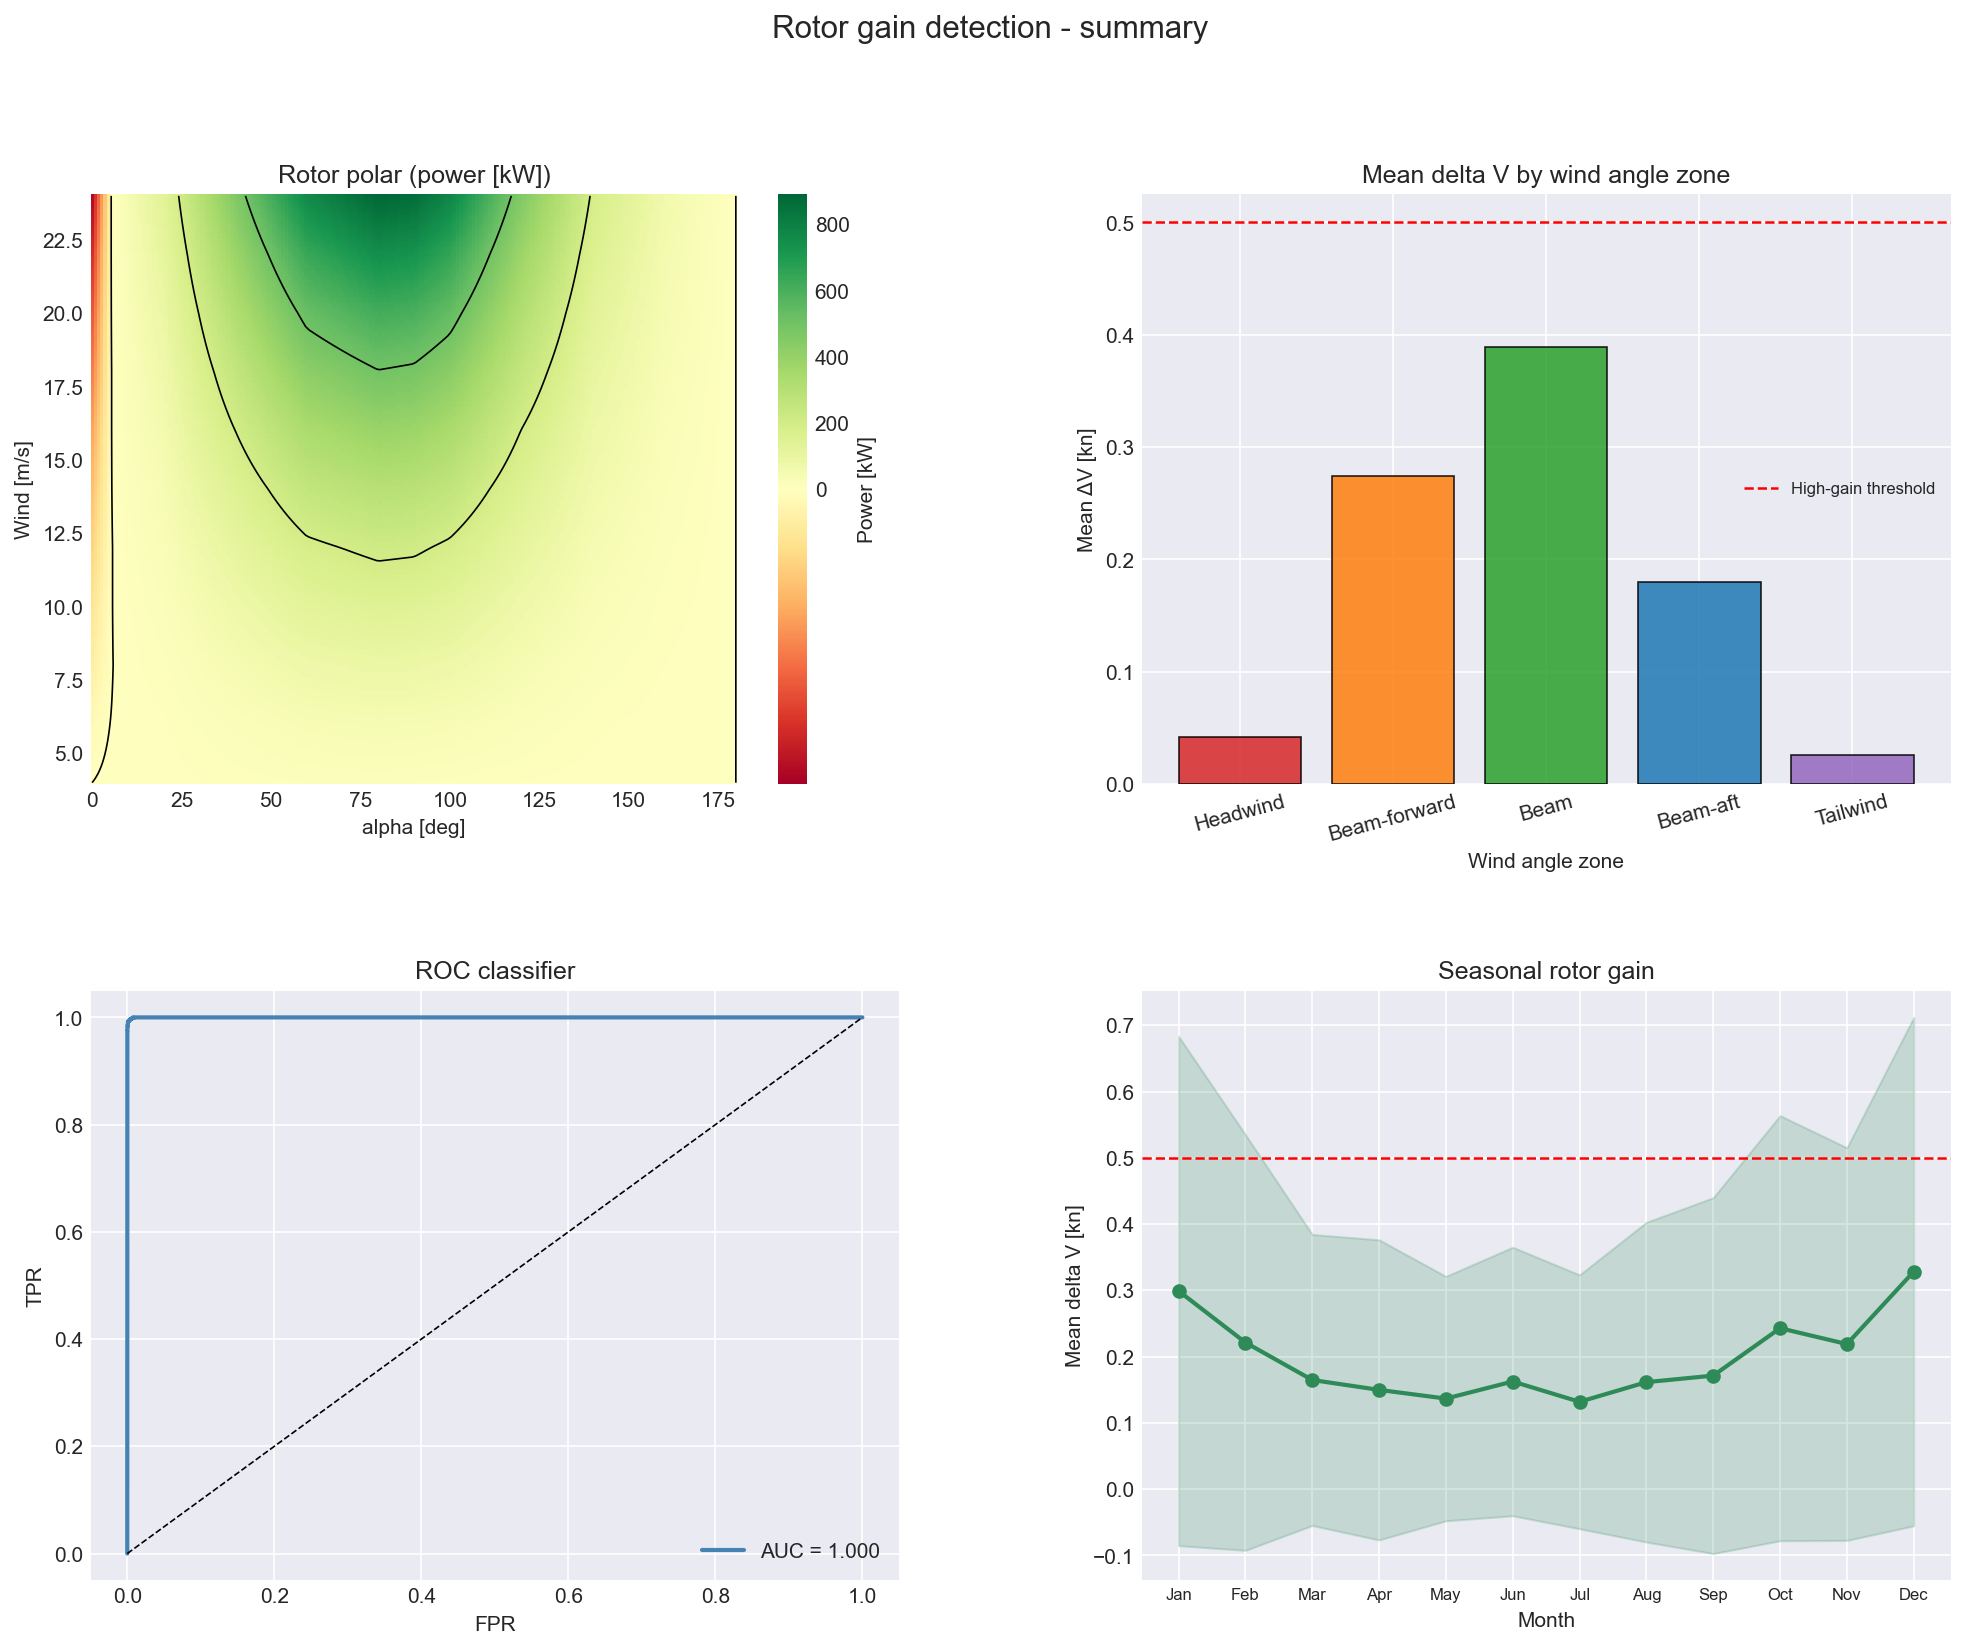
\includegraphics[width=\columnwidth, height=0.46\textheight, keepaspectratio]{rotor_gain_detection.png}
{\small Gain detection: high-gain ($\Delta$SOG $\geq 0.5$ kn) moment distribution.}
\end{column}
\begin{column}{0.43\textwidth}
\scriptsize
\textbf{High-gain moments} ($\Delta$SOG $\geq 0.5$ kn): 14,856 obs.\ = \textbf{11.9\%} of dataset. Median wind 11.5 m/s; median angle 82$^\circ$ (80\% between 50-113$^\circ$).

\vspace{0.1cm}
\textbf{XGBoost classifier}
\begin{center}
\begin{tabular}{lr}
\toprule
Accuracy & 99.8\% \\
Precision & 99.4\% \\
Recall & 99.0\% \\
F1 & 0.992 \\
ROC-AUC & 1.000 \\
\bottomrule
\end{tabular}
\end{center}

\vspace{0.05cm}
\textbf{Transparent rule}: wind $\geq$ 8 m/s \& angle 50-130$^\circ$ gives recall 95.8\%, accuracy 94.2\%. Easy to apply to forecasts on the bridge.

\begin{block}{Key takeaway}
Only 12\% of moments are high-gain, but they carry the bulk of rotor value - plan around them.
\end{block}
\end{column}
\end{columns}
\end{frame}

% ============================================================
%  PART 5 - UNCERTAINTY & CONCLUSIONS
% ============================================================

\sectiondivider{Part V}{Uncertainty \& Conclusions}{Hubert Jaczy\'nski}{Monte Carlo routing $\cdot$ Key findings $\cdot$ Operational takeaways}

%------------------------
\begin{frame}{Extension 5: Monte Carlo routing under uncertainty}
\begin{columns}
\begin{column}{0.54\textwidth}
\centering
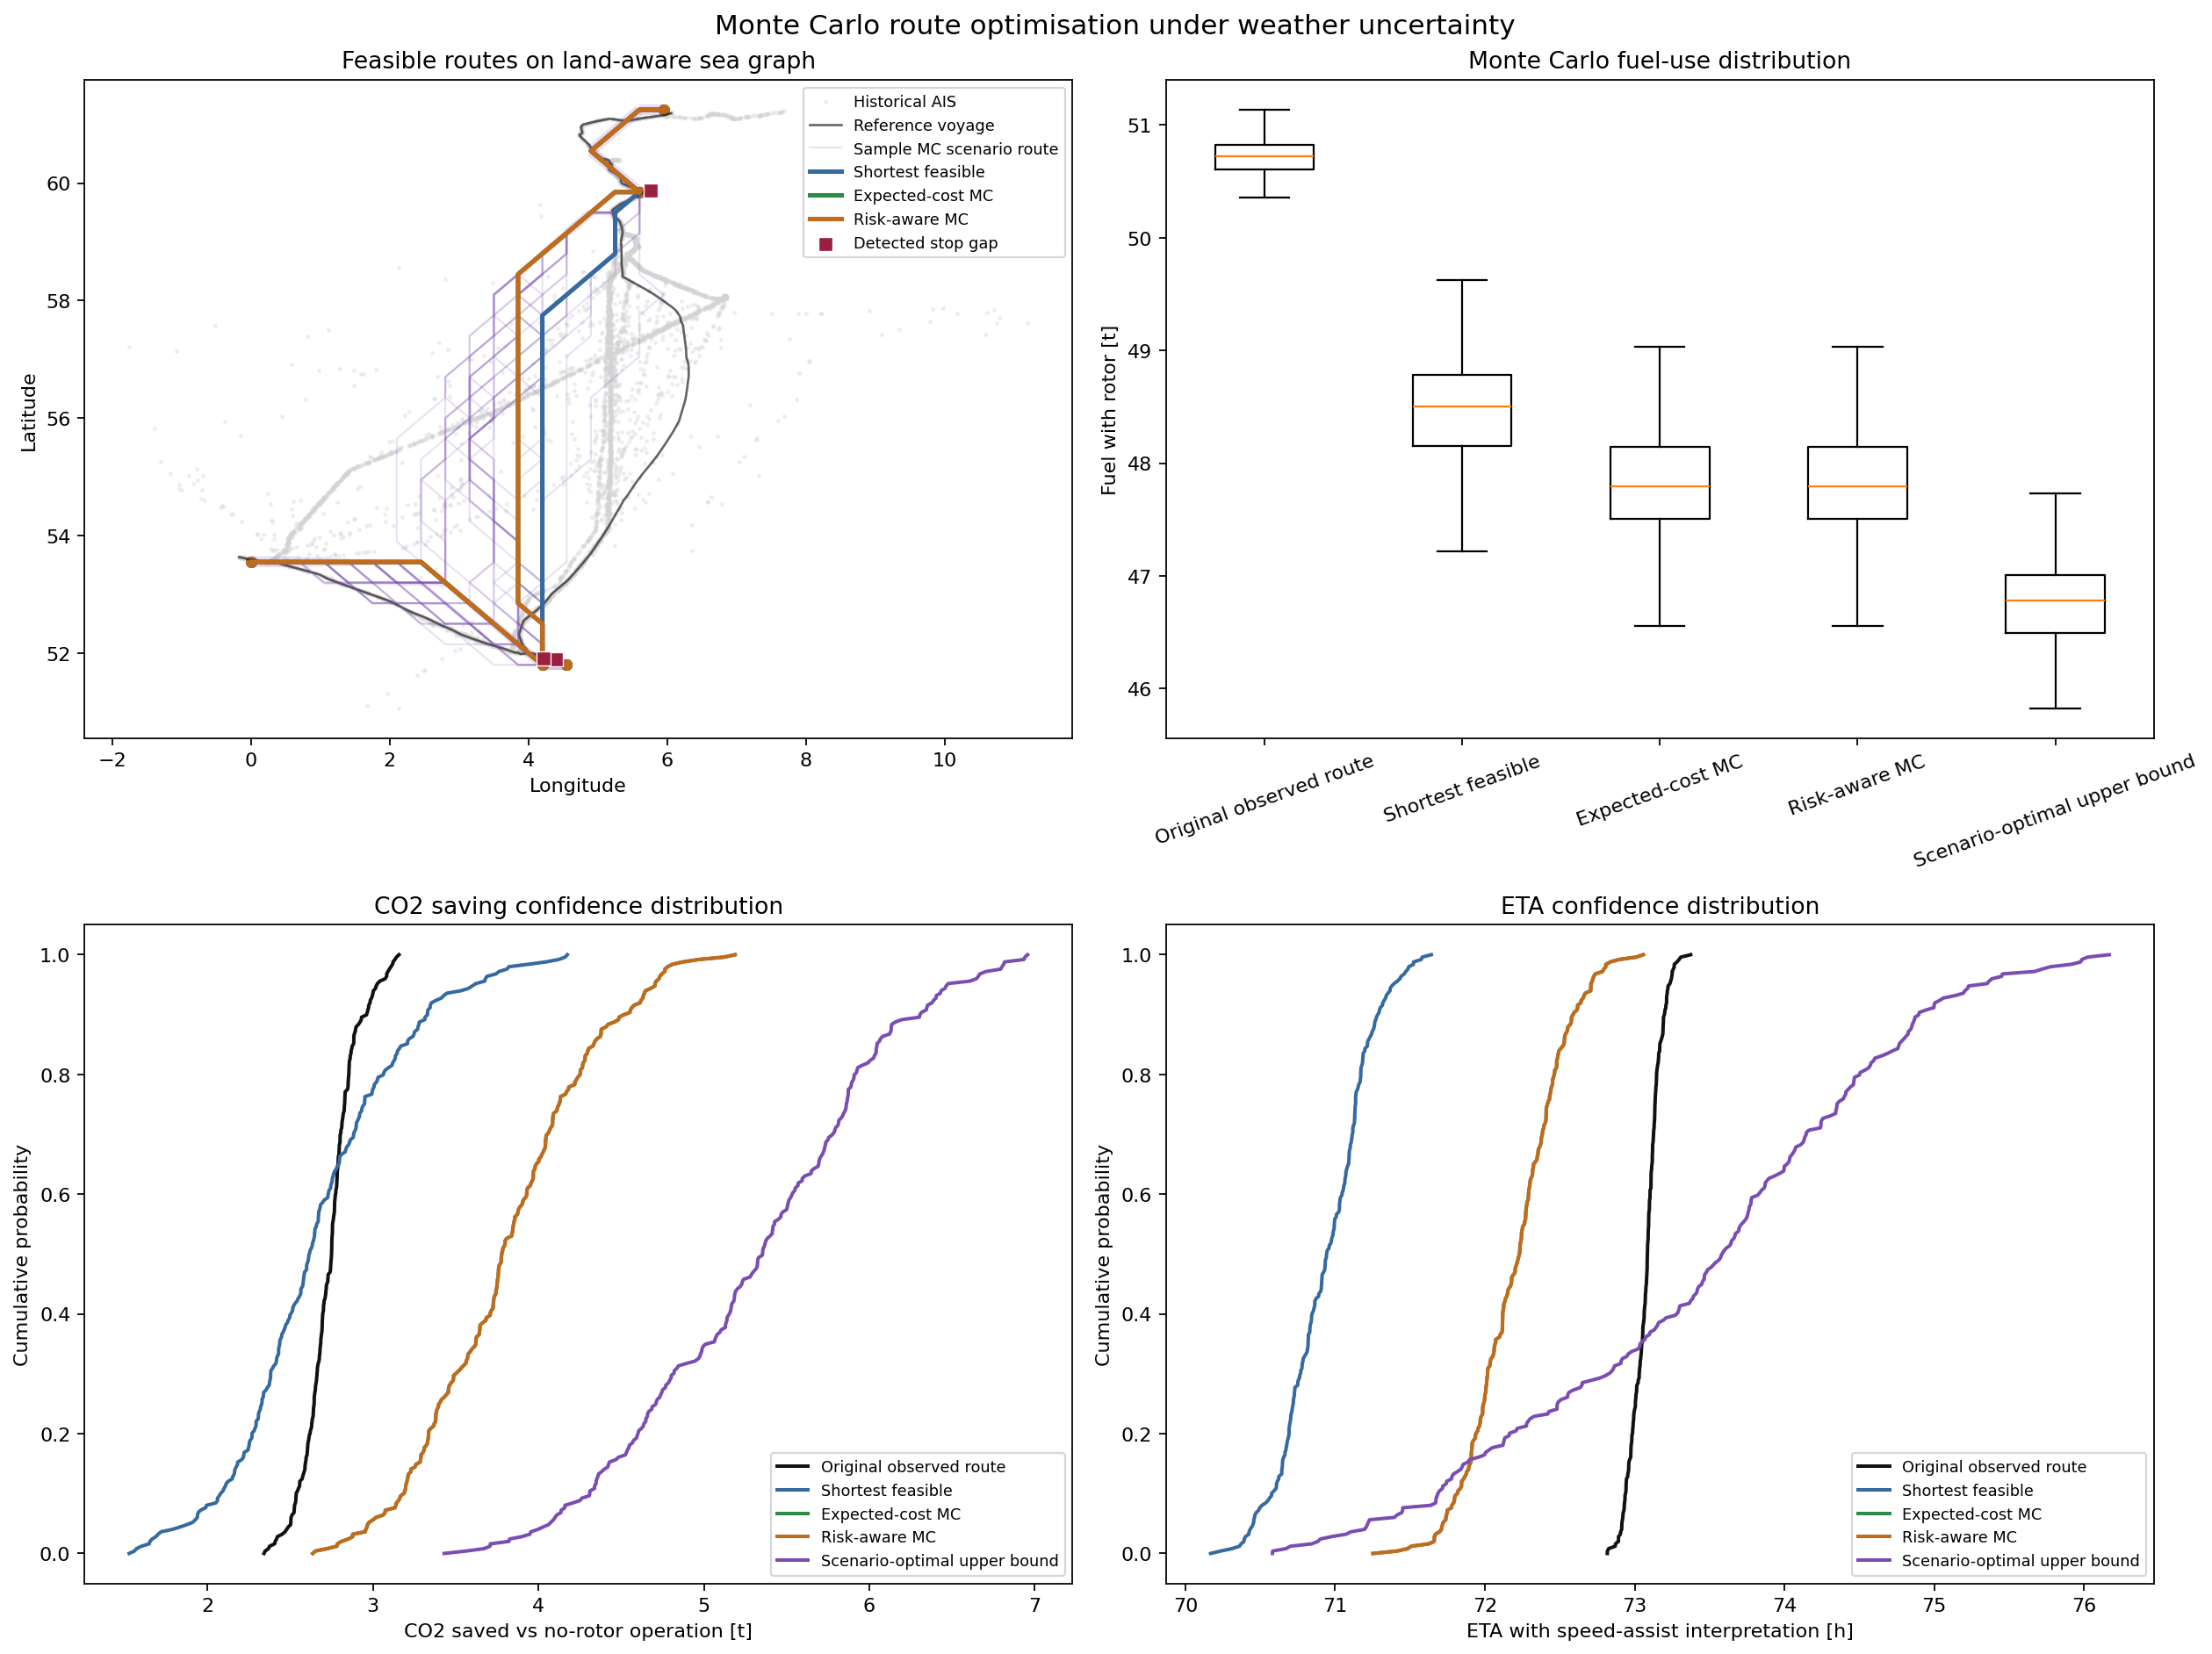
\includegraphics[width=\columnwidth, height=0.46\textheight, keepaspectratio]{monte_carlo_routing.png}
{\small Monte Carlo routing: 1,000 scenario samples for Voyage 364.}
\end{column}
\begin{column}{0.43\textwidth}
\scriptsize
\textbf{Voyage 364 - four route variants} (land-masked graph: 537 nodes, 3,784 edges)
\begin{center}
\begin{tabular}{lrr}
\toprule
\textbf{Route} & \textbf{Fuel (t)} & \textbf{Saved (t)} \\
\midrule
Observed & 50.72 & 0.88 \\
Shortest feasible & 48.47 & 0.86 \\
MC expected-cost & 47.81 & \textbf{1.22} \\
Scenario upper bd & 46.75 & \textbf{1.70} \\
\bottomrule
\end{tabular}
\end{center}

\vspace{0.05cm}
\begin{itemize}\setlength\itemsep{1pt}
  \item MC route beats shortest-feasible with \textbf{85.6\% probability}
  \item CO$_2$ saved: up to 5.3 t/voyage (upper bound)
  \item 4 itinerary legs, 3 detected port stops
\end{itemize}

\begin{block}{Key takeaway}
Uncertainty-aware routing outperforms greedy shortest path under rotor-gain objective.
\end{block}
\end{column}
\end{columns}
\end{frame}

% ============================================================
%  PART 6 - CONCLUSIONS
% ============================================================

%------------------------
\begin{frame}{Conclusion}
\footnotesize
\begin{columns}
\begin{column}{0.50\textwidth}
\textbf{Modelling}
\begin{itemize}
  \item Lagged nowcast XGBoost: MAE \textbf{0.406 kn}, $R^2$ \textbf{0.839} - strong short-horizon SOG prediction.
  \item Weather-only models are limited by missing operational variables (engine, draught, loading).
  \item Chronological voyage split prevents temporal leakage and tests real generalisation.
\end{itemize}
\vspace{0.15cm}
\textbf{Rotor scenario}
\begin{itemize}
  \item Mean speed uplift \textbf{0.202 kn}; weather-window coverage \textbf{+1.5 pp}.
  \item Only \textbf{11.9\%} of moments are high-gain - rotor is a conditional asset.
  \item Rule: wind $\geq$ 8 m/s at beam/quartering angle (50-130$^\circ$).
\end{itemize}
\end{column}
\begin{column}{0.47\textwidth}
\textbf{Operational impact (scenario estimates)}
\begin{itemize}
  \item 37.4 t fuel / 116 t CO$_2$ saved per year.
  \item CII improvement 53.75 $\to$ 53.20 g CO$_2$/(t nm).
  \item Westbound legs gain most from rotor assistance.
\end{itemize}
\vspace{0.15cm}
\textbf{What was built}
\begin{itemize}
  \item Reproducible pipeline: AIS + ERA5 + Copernicus Marine.
  \item Five extensions: energy, segmentation, routing, gain detection, Monte Carlo.
  \item Transparent assumptions throughout - auditable scenario, not a black-box claim.
\end{itemize}

\begin{block}{Final takeaway}
Wind-assisted propulsion is an opportunity map, not a constant bonus. The project identifies \textit{when} and \textit{where} it matters.
\end{block}
\end{column}
\end{columns}
\end{frame}

%------------------------
\begin{frame}[plain]
\centering
{\LARGE Thank you!}\\[0.4cm]
{\normalsize Questions welcome.}\\[0.3cm]
{\small Detailed methodology, assumptions, and extension figures follow in the appendix.}
\end{frame}

% ============================================================
%  APPENDIX
% ============================================================
\appendix

%------------------------
\begin{frame}[noframenumbering]{Appendix: prediction intervals (95\%)}
\centering
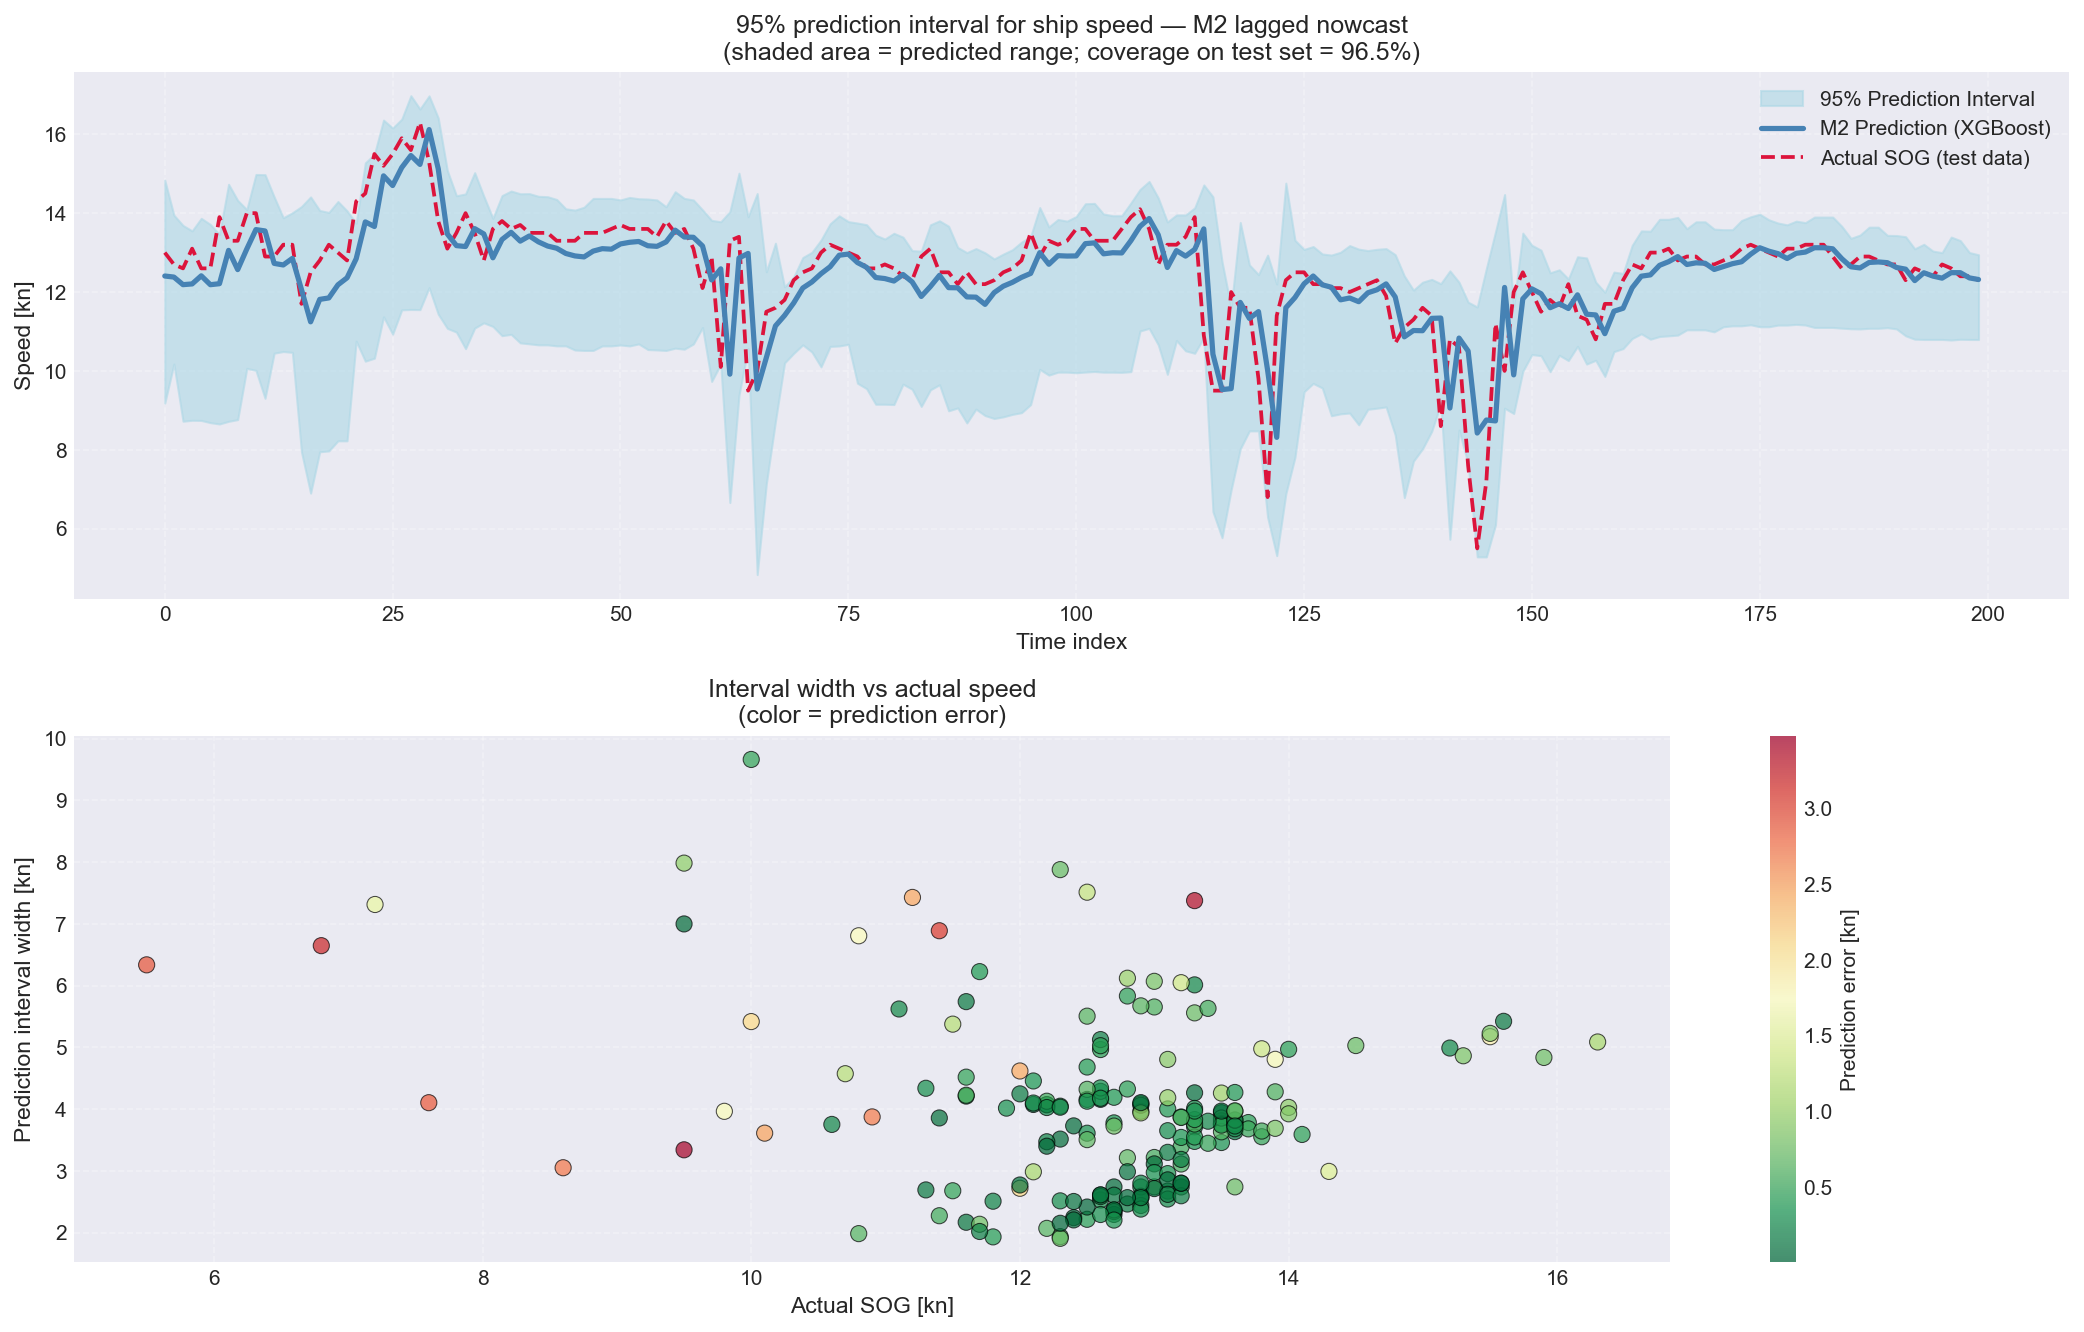
\includegraphics[width=0.88\textwidth, height=0.62\textheight, keepaspectratio]{prediction_intervals_95percent.png}

\vspace{0.1cm}
{\small 95\% quantile-regression prediction intervals for the nowcast model. Mean width 3.161 kn; empirical coverage 96.5\% on the test set - slightly conservative but well calibrated.}
\end{frame}

%------------------------
\begin{frame}[noframenumbering]{Appendix: rotor polar and seasonal variation}
\begin{columns}
\begin{column}{0.48\textwidth}
\centering
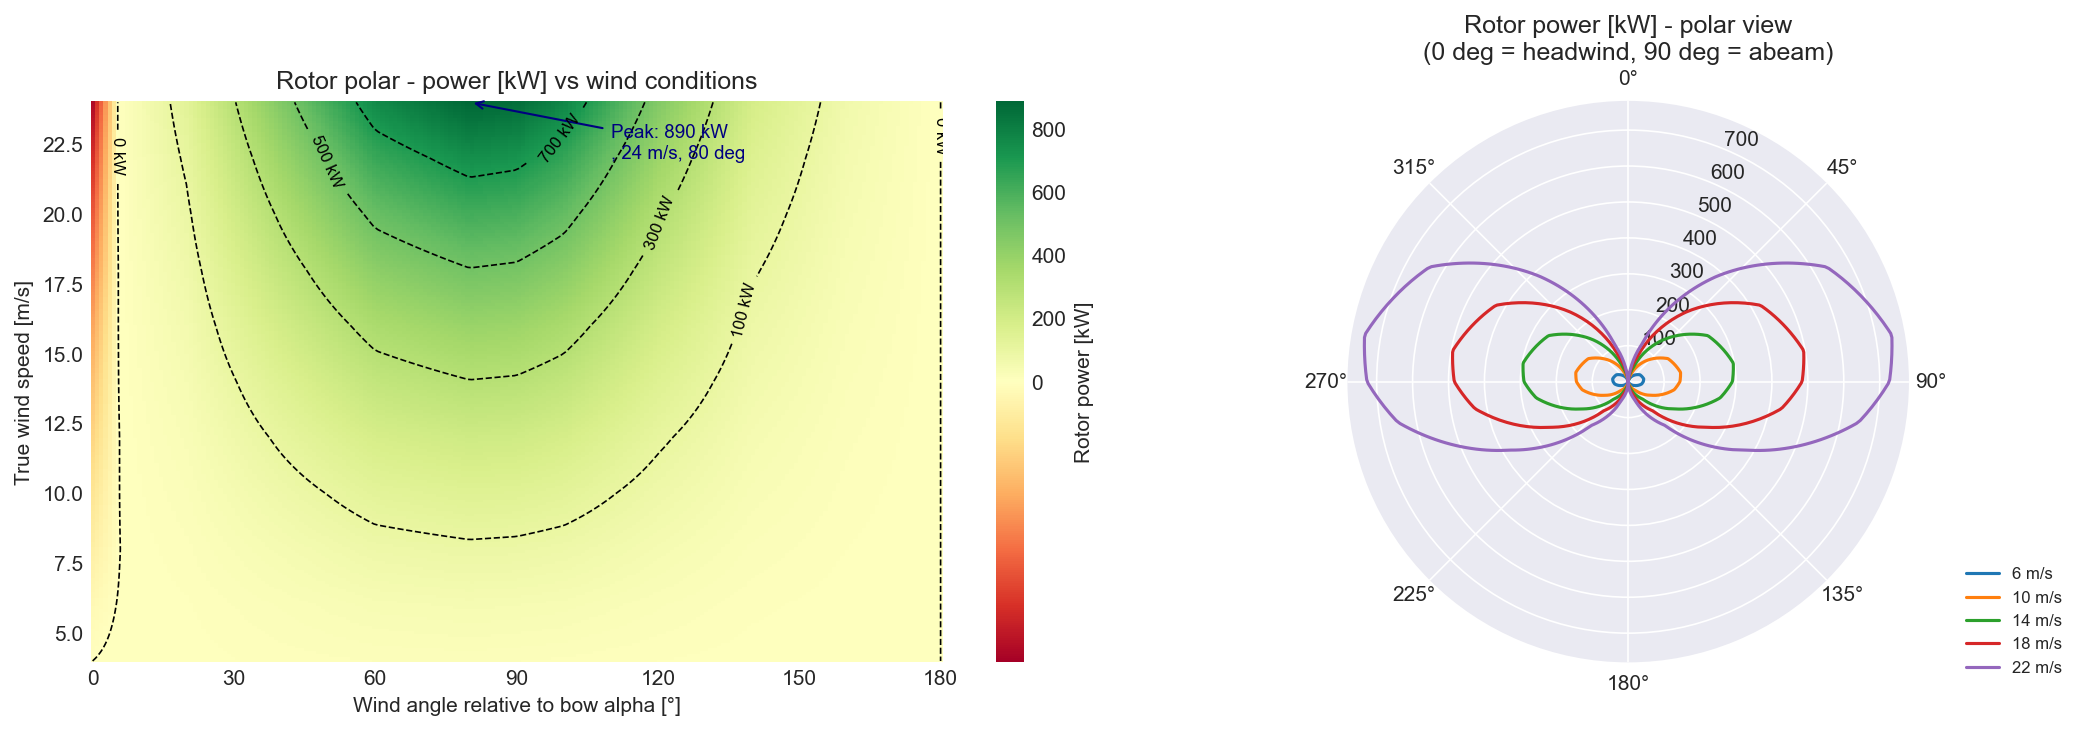
\includegraphics[width=\columnwidth, height=0.52\textheight, keepaspectratio]{rotor_polar.png}
{\small Rotor polar gain diagram.}
\end{column}
\begin{column}{0.48\textwidth}
\centering
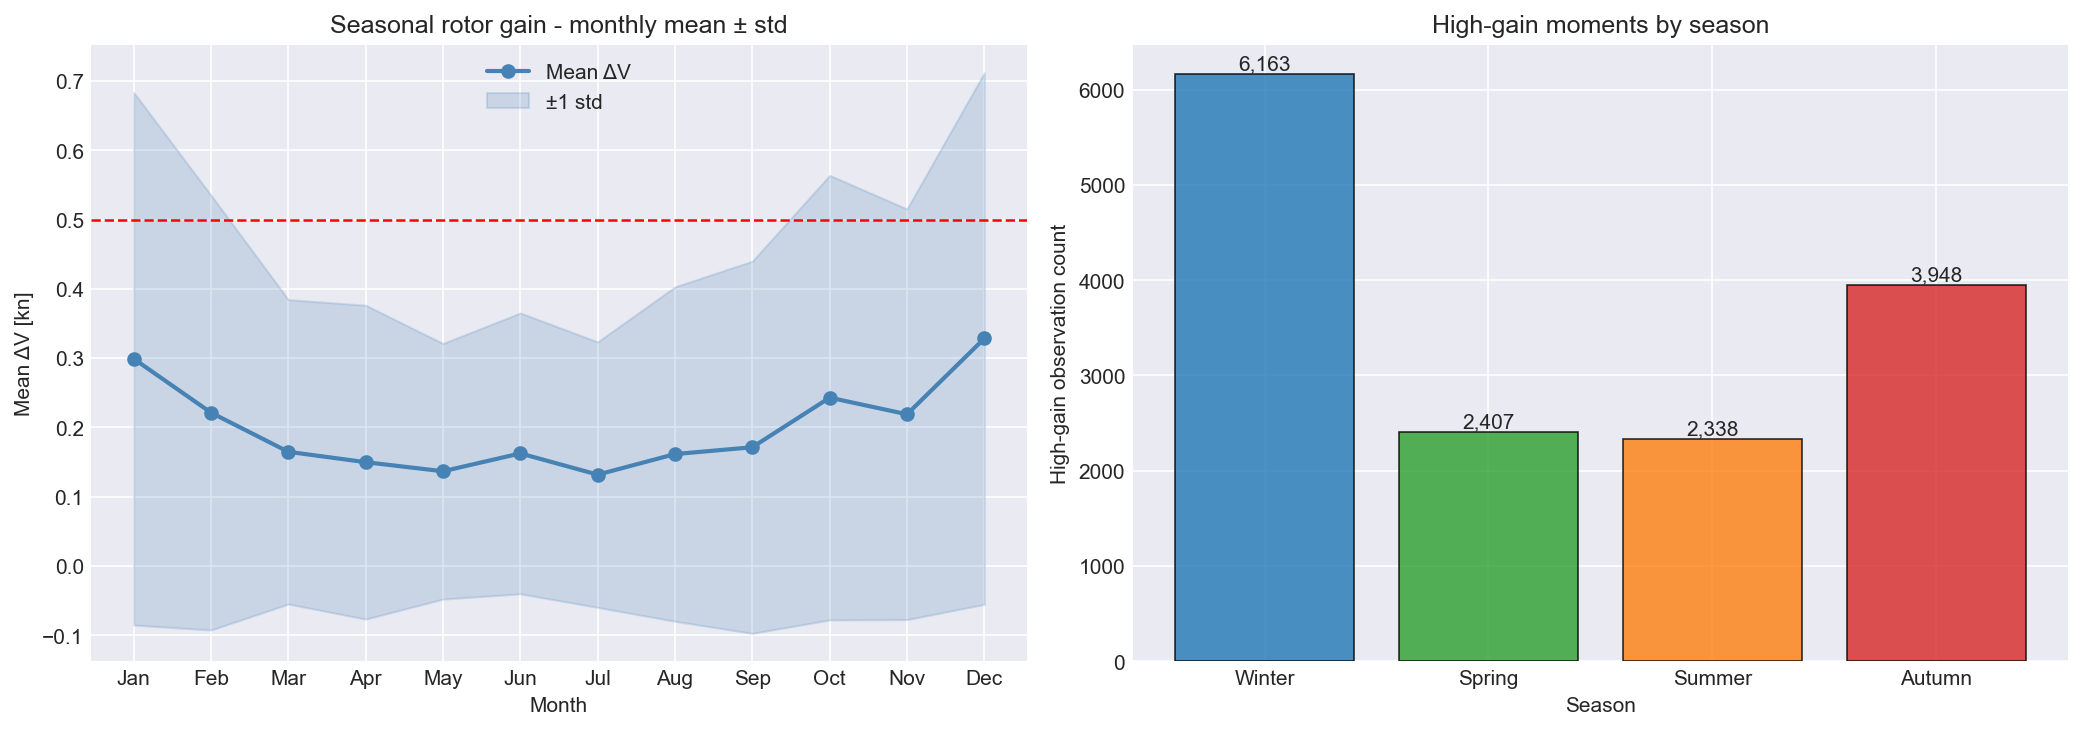
\includegraphics[width=\columnwidth, height=0.52\textheight, keepaspectratio]{rotor_seasonal.png}
{\small Seasonal rotor gain variation. December best (59.8 kW), July worst (26.6 kW). Winter wind is stronger but wave risk is higher.}
\end{column}
\end{columns}
\end{frame}

%------------------------
\begin{frame}[noframenumbering]{Appendix: rotor opportunity by voyage}
\begin{columns}
\begin{column}{0.48\textwidth}
\centering
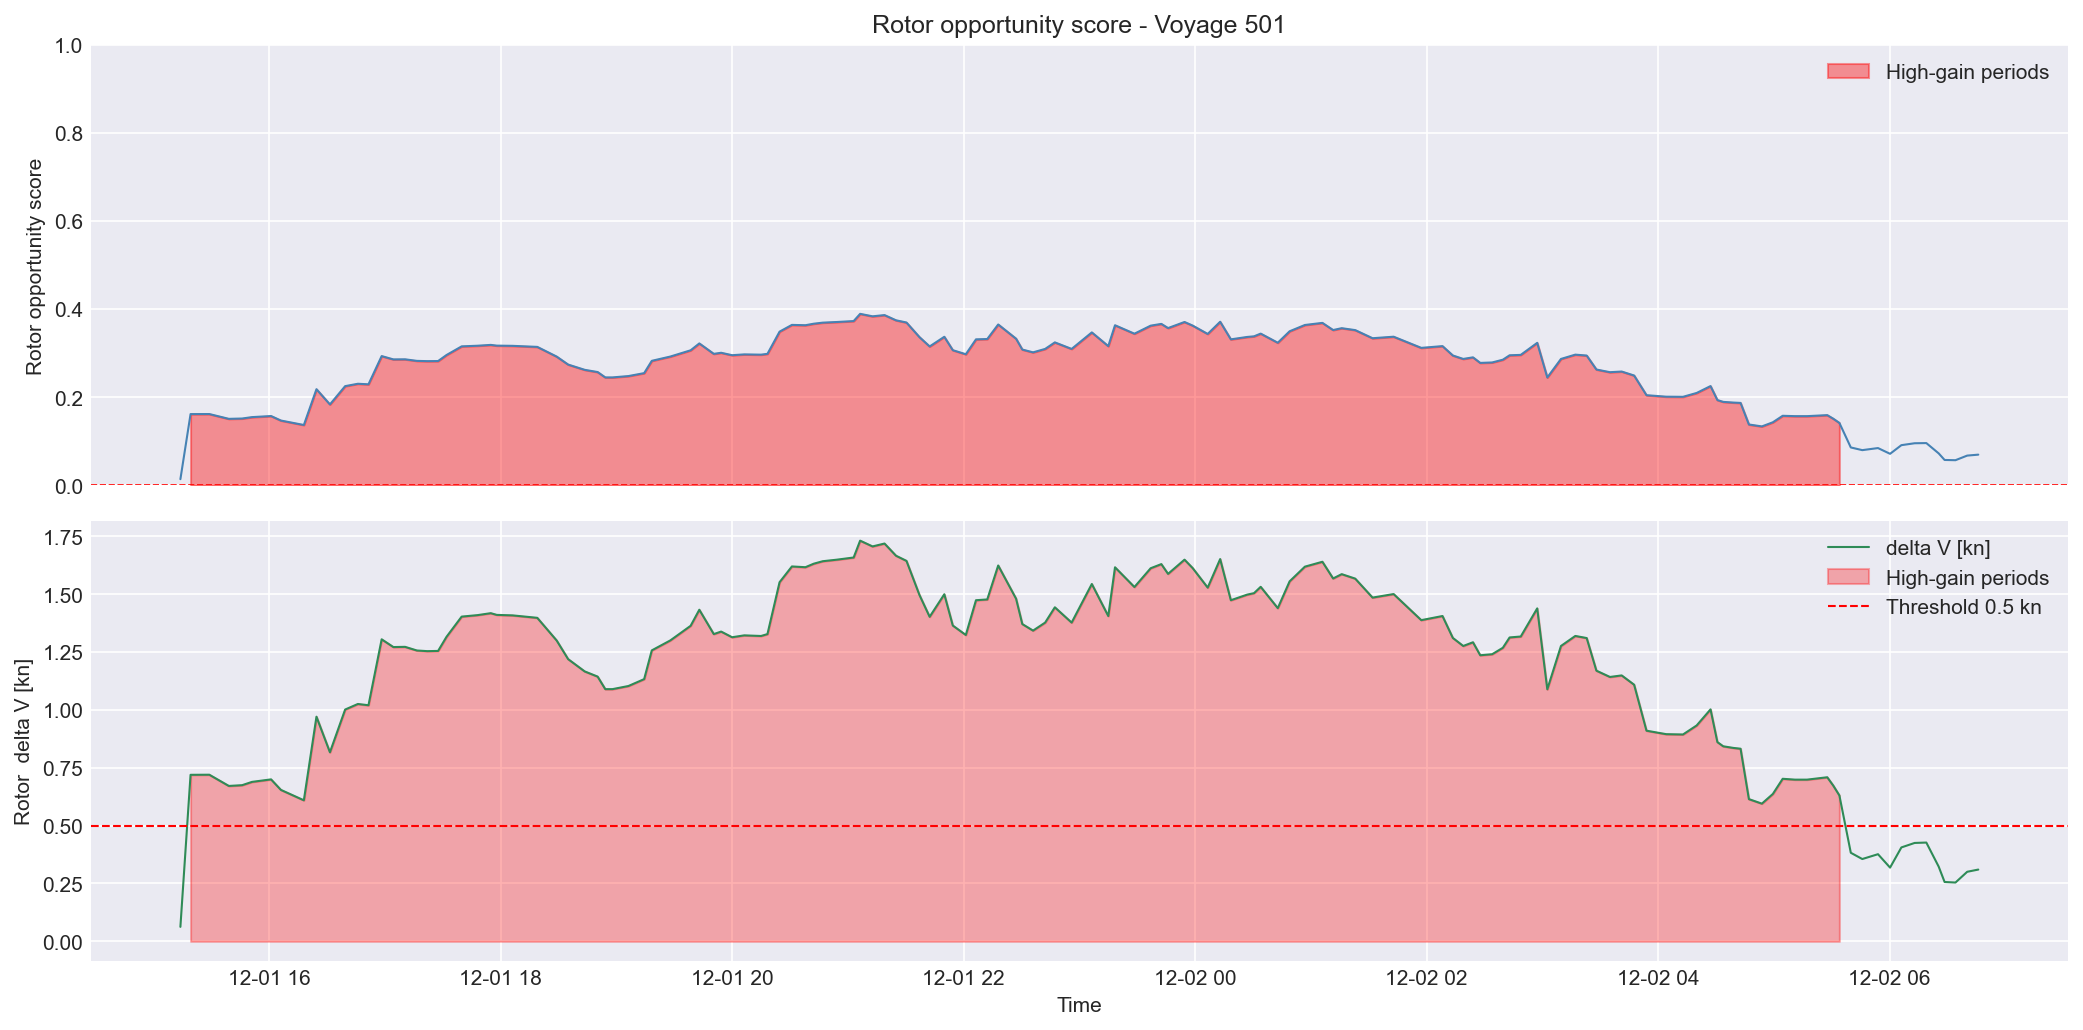
\includegraphics[width=\columnwidth, height=0.52\textheight, keepaspectratio]{rotor_opportunity_voyage501.png}
{\small Voyage 501: rotor opportunity map along the track.}
\end{column}
\begin{column}{0.48\textwidth}
\centering
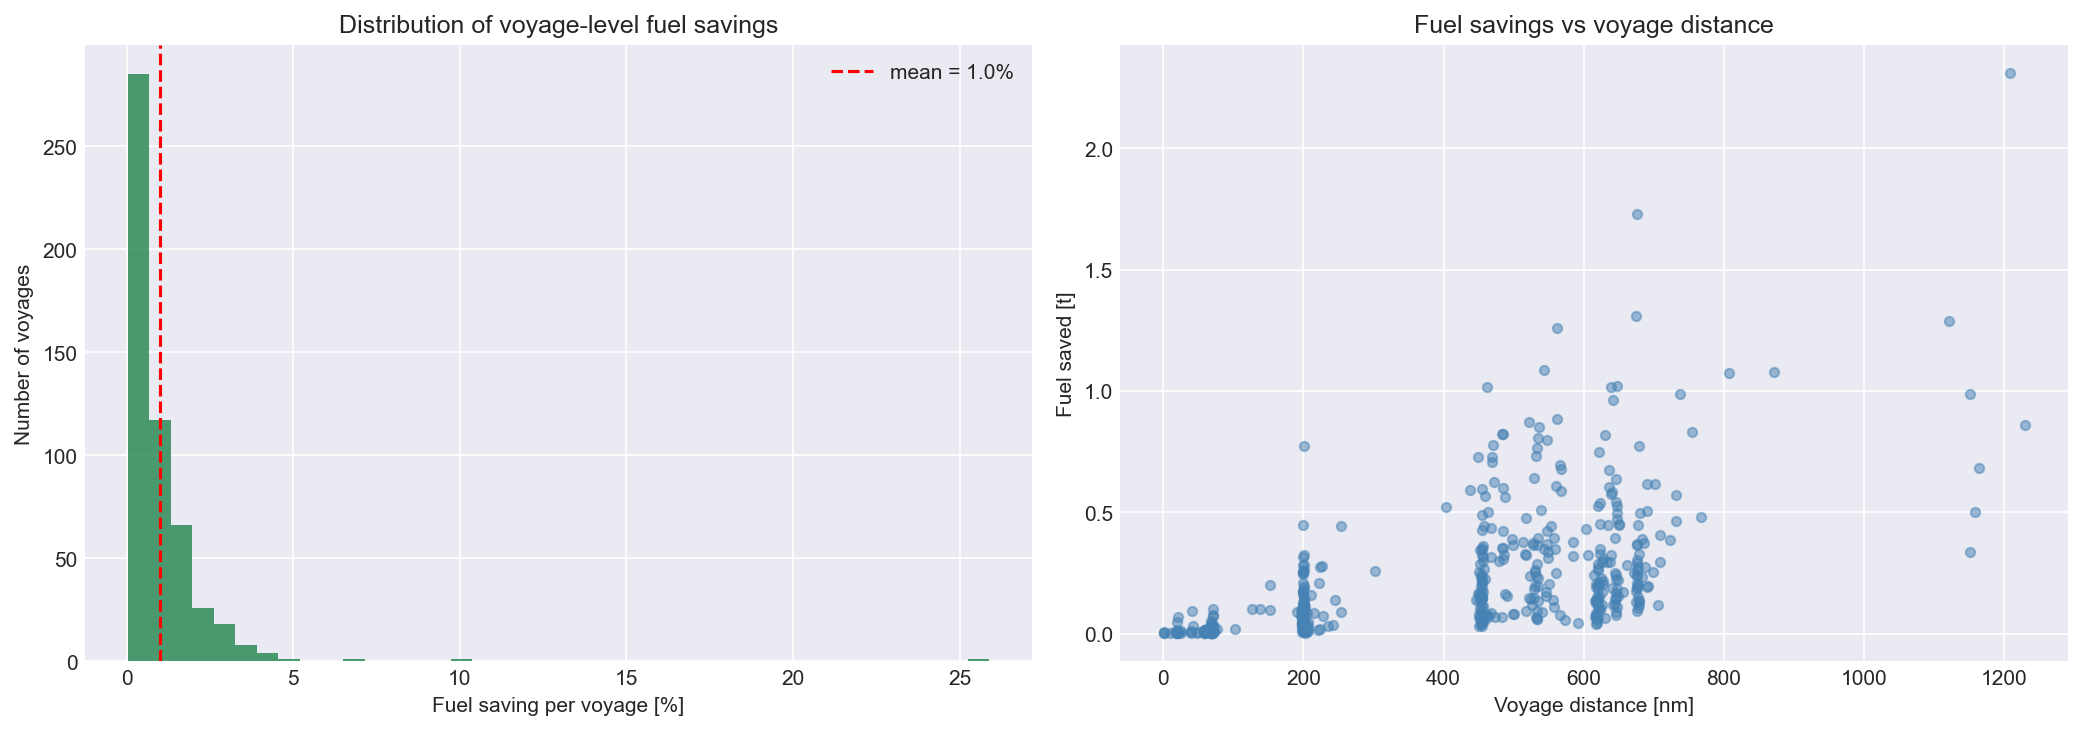
\includegraphics[width=\columnwidth, height=0.52\textheight, keepaspectratio]{voyage_fuel_savings.png}
{\small Per-voyage fuel savings distribution.}
\end{column}
\end{columns}
\end{frame}

%------------------------
\begin{frame}[noframenumbering]{Appendix: rotor gain decision map and classifier}
\begin{columns}
\begin{column}{0.49\textwidth}
\centering
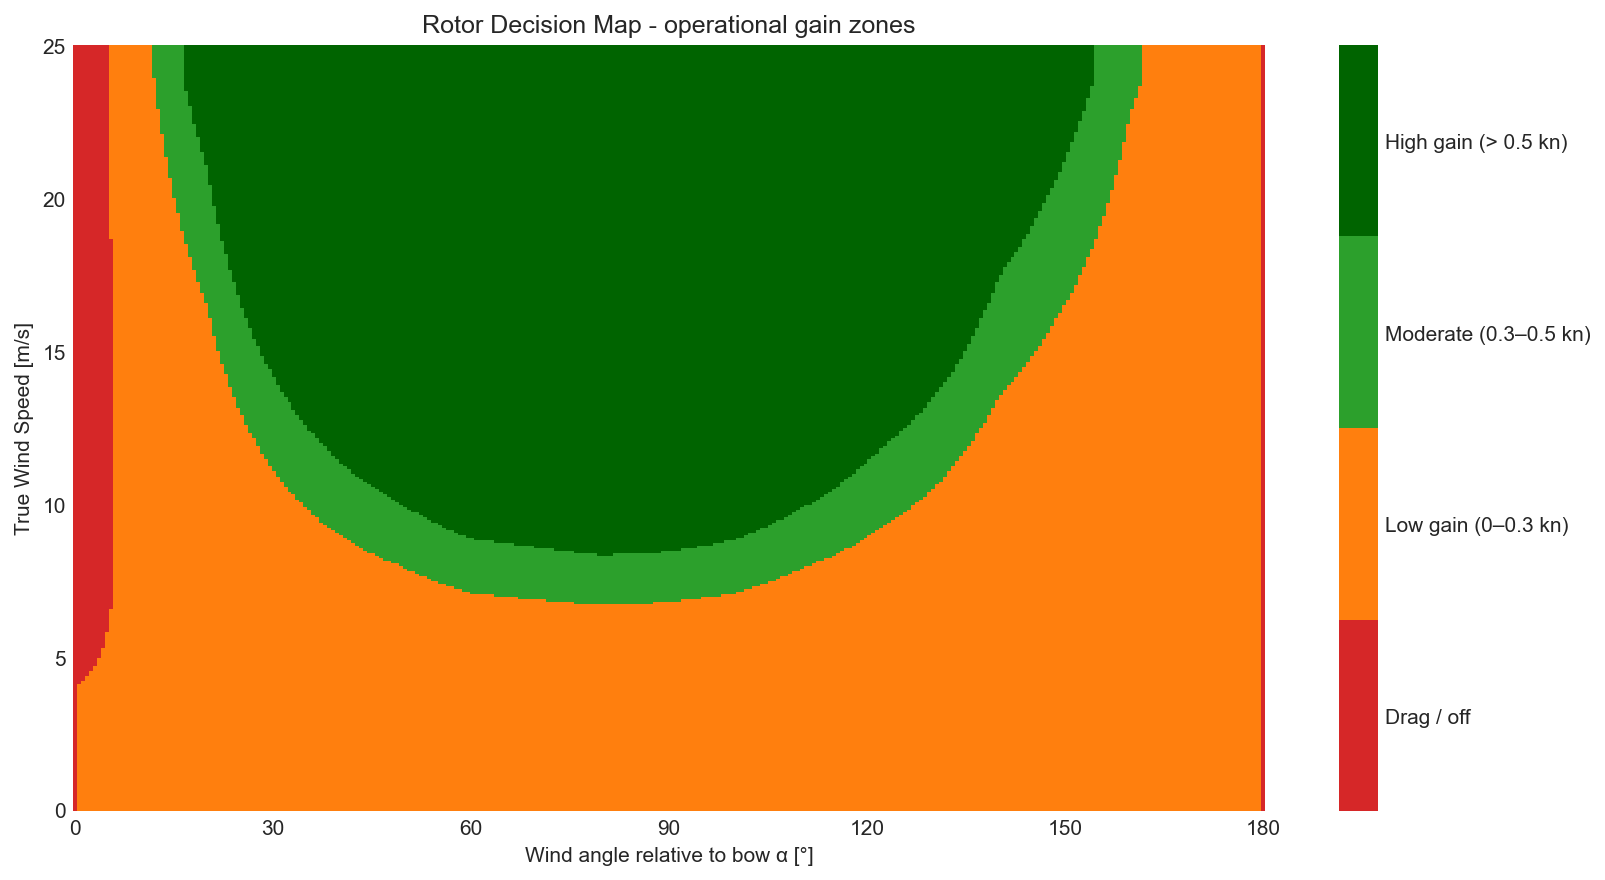
\includegraphics[width=\columnwidth, height=0.54\textheight, keepaspectratio]{rotor_decision_map.png}
{\small Rule-based high-gain zones.}
\end{column}
\begin{column}{0.49\textwidth}
\centering
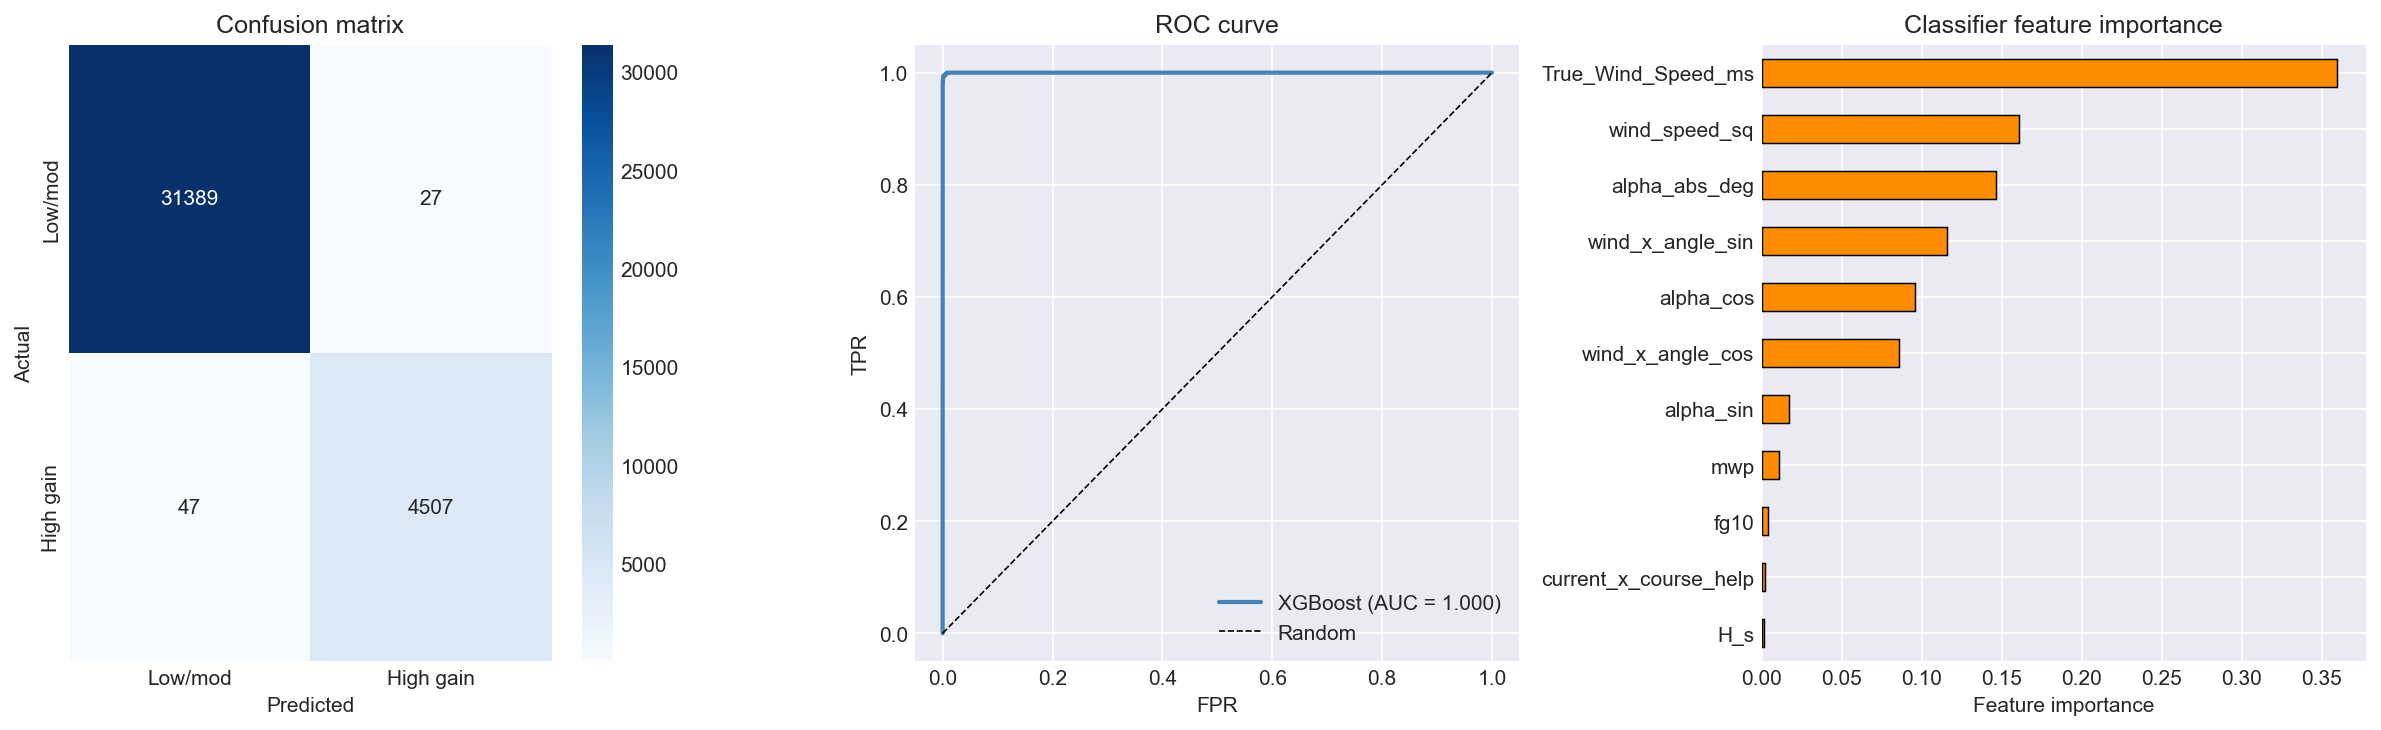
\includegraphics[width=\columnwidth, height=0.54\textheight, keepaspectratio]{rotor_classifier.png}
{\small XGBoost classifier confusion matrix and ROC.}
\end{column}
\end{columns}
\end{frame}

%------------------------
\begin{frame}[noframenumbering]{Appendix: rotor wave-height interaction}
\centering
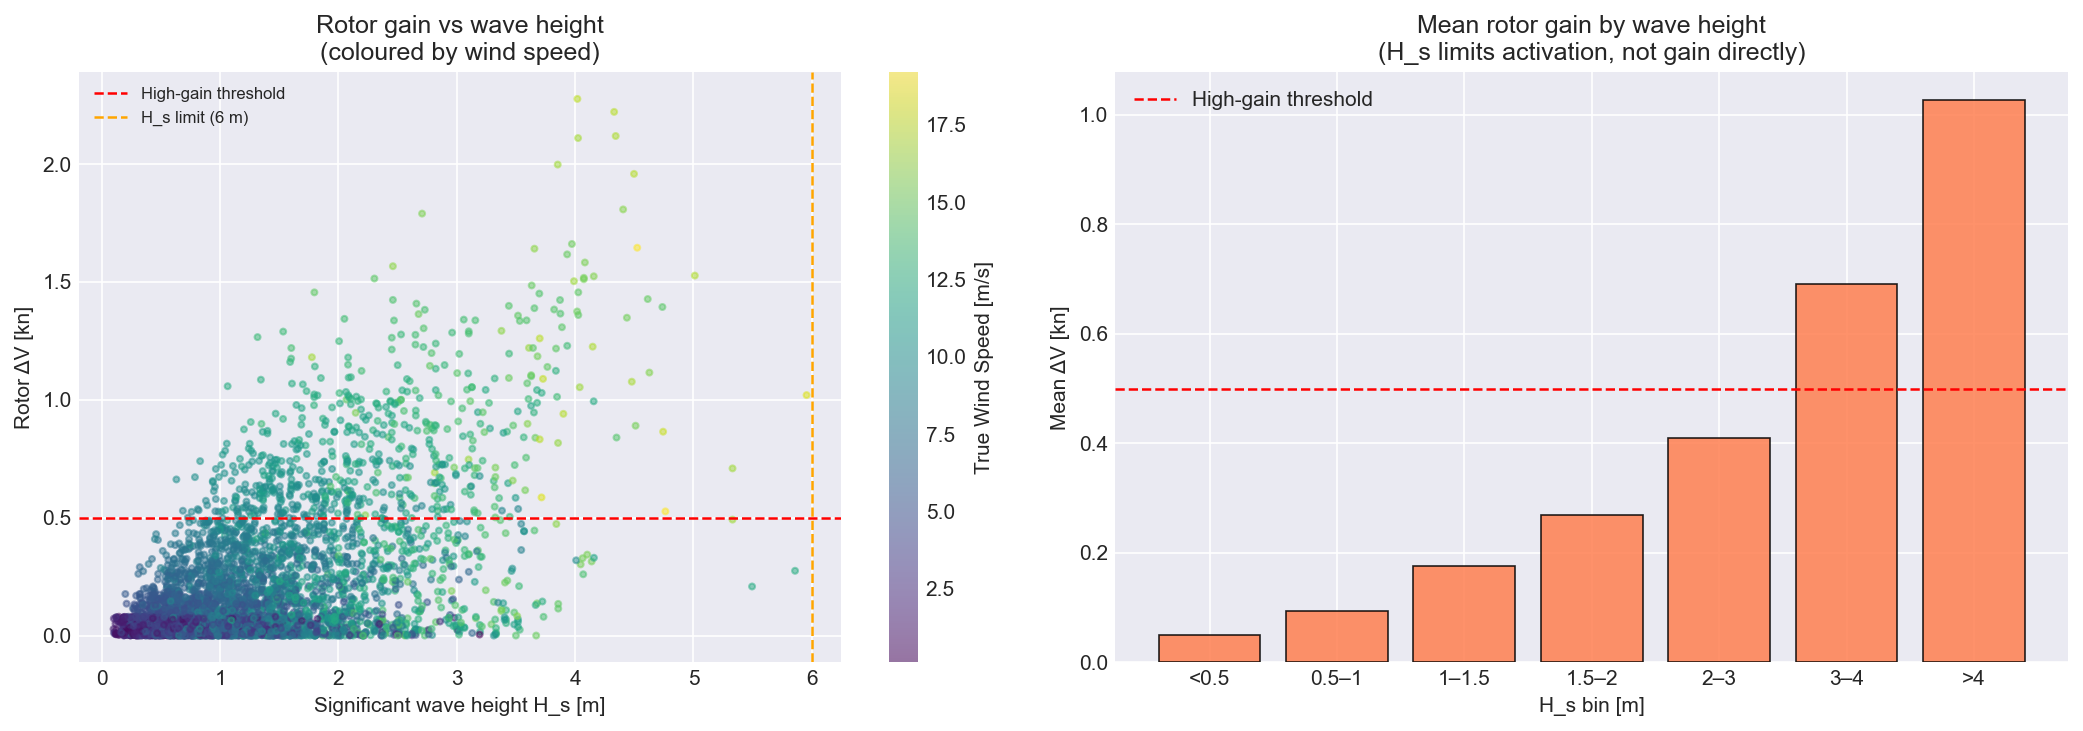
\includegraphics[width=0.88\textwidth, height=0.62\textheight, keepaspectratio]{rotor_hs_interaction.png}

\vspace{0.1cm}
{\small Wave height interaction with rotor gain. $H_s$ primarily acts as an operational gate (rotor off above 6 m); it is not the main driver of gain magnitude. Wind angle and wind speed create the opportunity; sea state can remove it.}
\end{frame}

%------------------------
\begin{frame}[noframenumbering]{Appendix: model comparison and zone analysis}
\begin{columns}
\begin{column}{0.49\textwidth}
\centering
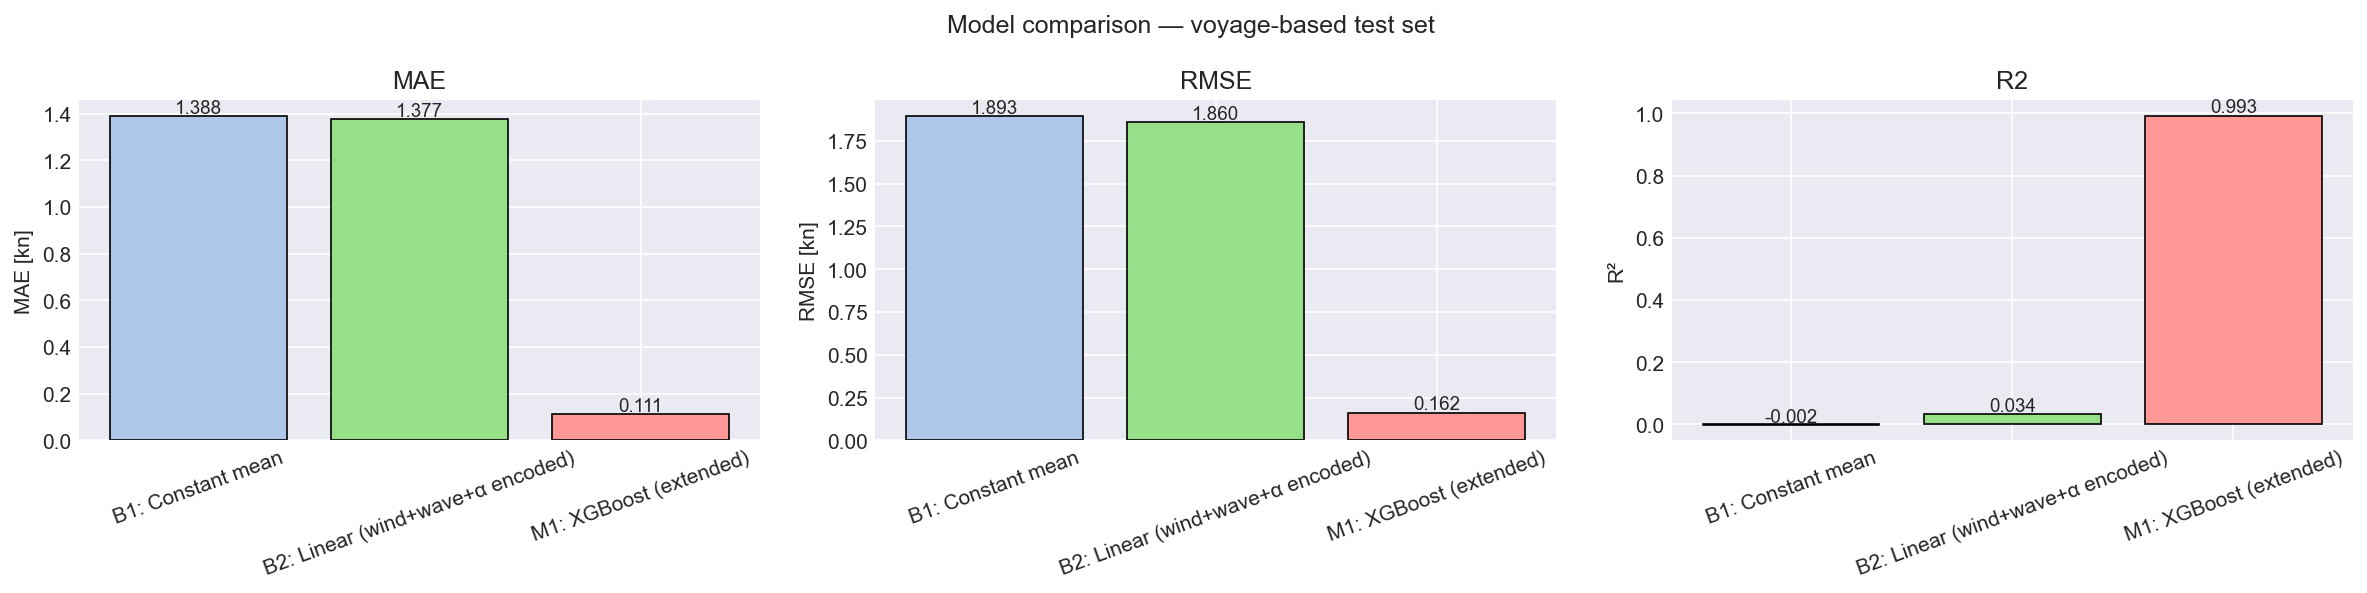
\includegraphics[width=\columnwidth, height=0.54\textheight, keepaspectratio]{model_comparison.png}
{\small All four model MAE/RMSE/$R^2$ side-by-side.}
\end{column}
\begin{column}{0.49\textwidth}
\centering
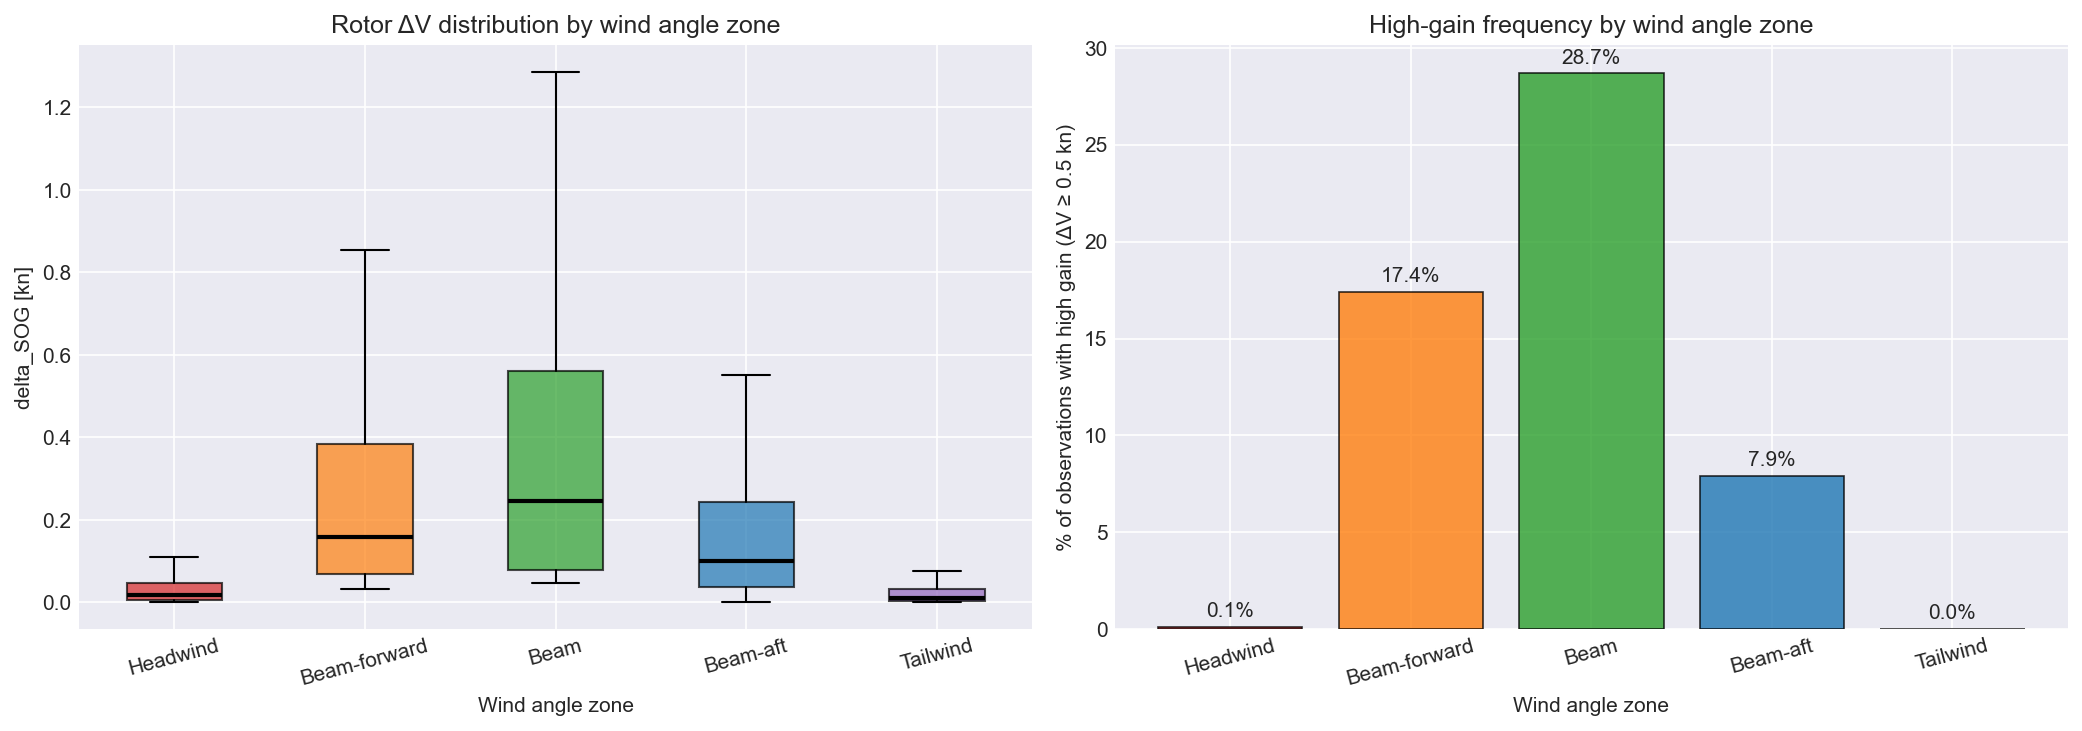
\includegraphics[width=\columnwidth, height=0.54\textheight, keepaspectratio]{rotor_zone_analysis.png}
{\small Rotor zone analysis across the study area.}
\end{column}
\end{columns}
\end{frame}

%------------------------
\begin{frame}[noframenumbering]{Appendix: rotor scenario methodology - full formula}
\small
\textbf{Rotor power from polar table}:
\[
  P_\text{rotor} = f_\text{polar}(U_\text{wind},\, |\alpha|)
\]
where $|\alpha|$ is the absolute relative wind angle (0 = headwind, 90 = beam).

\textbf{Active condition}:
\[
  \text{active} = \mathbf{1}\bigl[P_\text{rotor}>0\bigr]\cdot\mathbf{1}\bigl[H_s \leq 6\,\text{m}\bigr]\cdot\mathbf{1}\bigl[U_\text{wind} \leq 42\,\text{m/s}\bigr]
\]

\textbf{Speed contribution}:
\[
  \Delta\text{SOG} = \text{active} \times \frac{P_\text{rotor}}{200\,\text{kW/kn}}
\]

\textbf{Fuel saving rate} (cubic resistance model):
\[
  \dot{m}_\text{fuel} = \frac{P_\text{brake} \cdot \text{SFOC}}{1000}
  \quad\text{where}\quad
  P_\text{brake} = P_\text{design}\left(\frac{\text{SOG}}{v_\text{design}}\right)^3 - P_\text{rotor}
\]

\begin{block}{Design principle}
Rotor variables are a \emph{scenario overlay} applied after prediction - the baseline model trains on observed operations only, keeping prediction and scenario logics cleanly separated.
\end{block}
\end{frame}

\end{document}
